\documentclass[12pt]{article}

\usepackage[margin=1.0in]{geometry}
\usepackage[parfill]{parskip}
\usepackage{changepage}
\usepackage{amsmath}
\usepackage[font=bf]{caption}
\usepackage{subcaption} 
\usepackage{graphicx}
\usepackage{adjustbox}
\usepackage{url}
\usepackage{xcolor}

\usepackage[numbib]{tocbibind}



\begin{document}

\setlength{\parskip}{12pt}      % set paragraph skipping to one whole line



\begin{titlepage}
    \begin{center}
        \vspace*{\fill}
        
        \huge
        A Kalman Filter for Bluetooth RSSI Tracking
        
        \vspace{36pt}

        \large
        Robert S. Huston

        \vspace{36pt}
        
        \today
        
        \vfill
    \end{center}
\end{titlepage}



\begin{abstract}
This article investigates the application of a Kalman filter for estimating Bluetooth
RSSI signal levels acquired via a mobile device. Three process models are explored:
Gauss-Markov, Gauss-Markov with random bias, and integrated Gauss-Markov. Experimental
data captured using an iPhone is used to demonstrate and compare the performance of each
model.
\end{abstract}



\clearpage
\tableofcontents



%-------------------------------------------------------------------------------
%
% Introduction
%
%-------------------------------------------------------------------------------

\clearpage
\section{Introduction}

Two basic architectures are representative of the reception of digital signals:
direct-conversion and low-IF. The basic direct-conversion architecture is shown in
Figure \ref{fig:rx-arch-direct}. The direct-conversion architecture supplies the baseband
I and Q digital samples directly to the DSP.

\begin{figure}[ht]
    \centering
    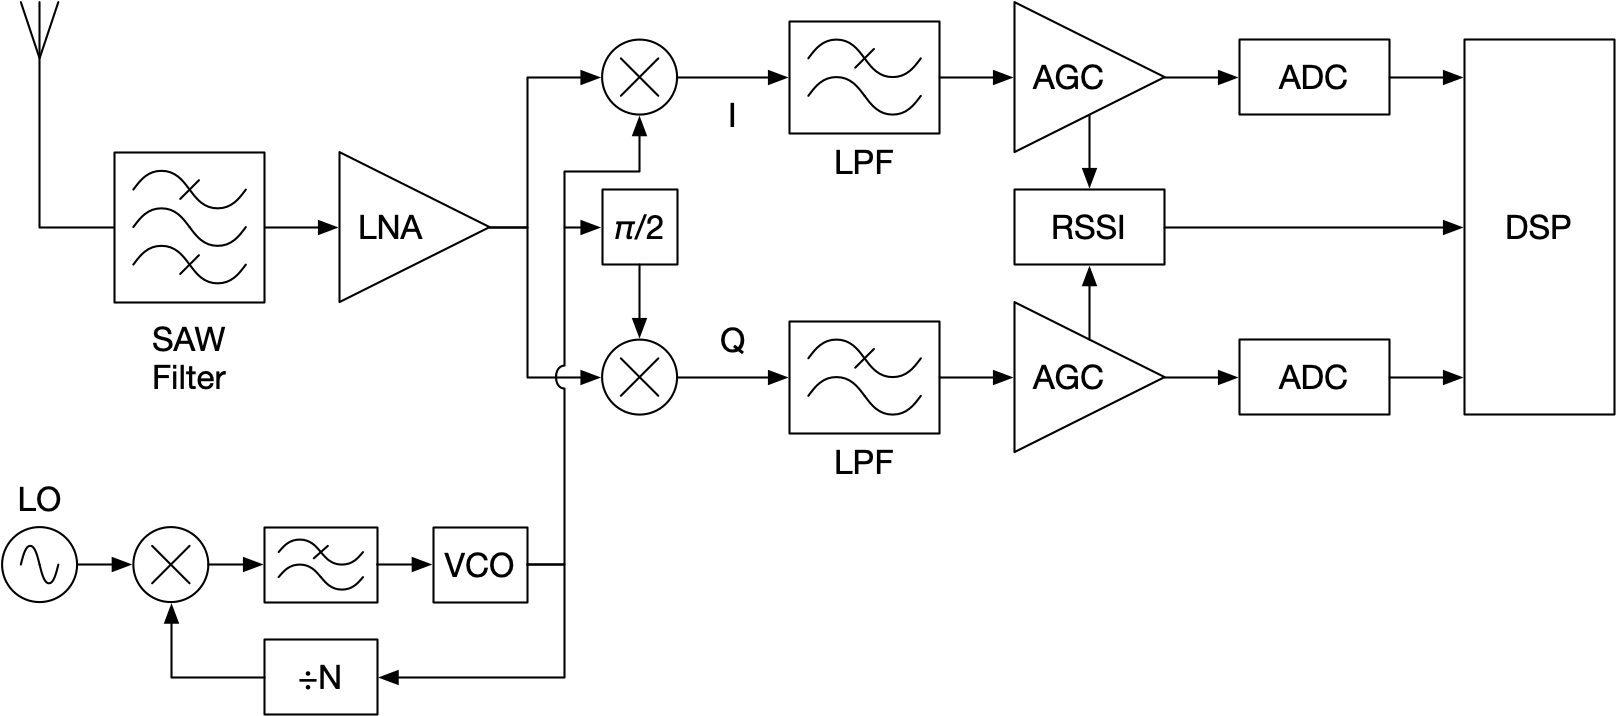
\includegraphics[width=1.0\textwidth]{RX-Arch-Direct.png}
    \caption{Digital Receiver Architecture - Direct Conversion}
    \label{fig:rx-arch-direct}
\end{figure}

The basic low-IF architecture is shown in Figure \ref{fig:rx-arch-low-if}. The low-IF
architecture supplies the IF digital samples to the DSP.

\begin{figure}[ht]
    \centering
    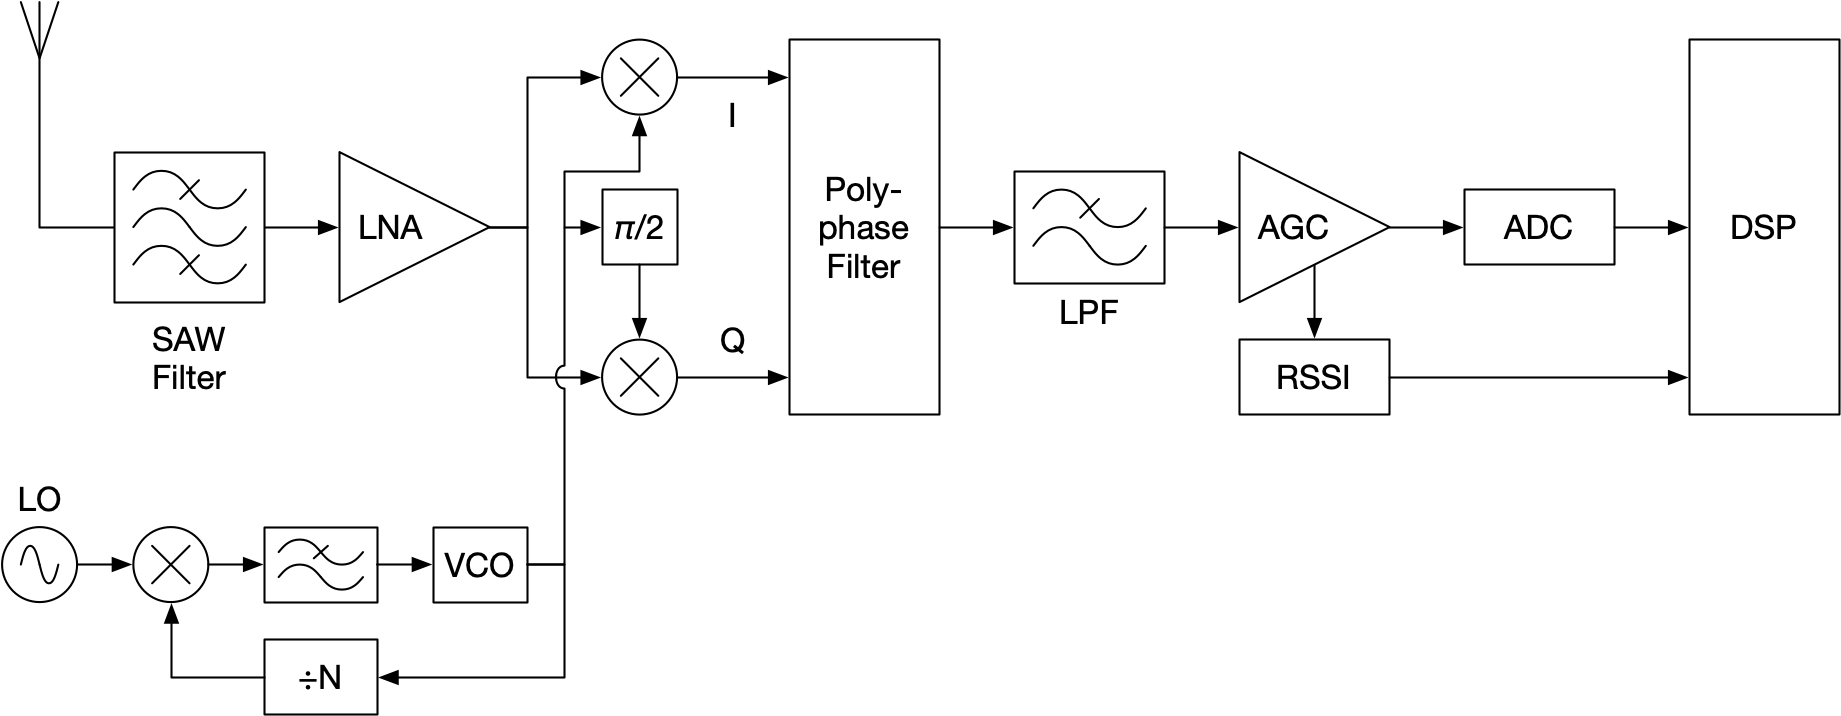
\includegraphics[width=1.0\textwidth]{RX-Arch-Low-IF.png}
    \caption{Digital Receiver Architecture - Low IF}
    \label{fig:rx-arch-low-if}
\end{figure}

While there are various engineering reasons for choosing one architecture over the other,
the main point to realize is that the RSSI measurement is typically related to the AGC
levels of the receiver. Because the AGC is constantly adjusting its gain in order to
track the incoming signal, the RSSI measurement as relayed by the signal processor will
fluctuate. In addition, the quality of the RSSI signal is highly dependent on both the
AGC operation as well as the processing strategies and algorithms implemented in the DSP.
Of course, the position of the radio antenna itself also has an effect on signal quality
due to shadowing and polarization, and also due to multipath signals imposed by the
physical layout of an indoor environment.

The reality is that Bluetooth RSSI measurements as acquired by a mobile device can be
highly erratic and can be quite unreliable in their raw form. The application of a filter
to refine the raw measurements is certainly warranted. In this paper, we explore the use
of three Kalman filter models for refining the RSSI measurement of a mobile device into
a more meaningful value.

We first explore the use a Gauss-Markov process to model the RSSI acquisition behavior of
a Bluetooth device signal as seen by the mobile device. We choose this model because its
autocorrelation function seems to match what we have observed from the signal behavior of
experimental RSSI data captured over time, and because the resulting Kalman filter is
scalar. We then present two experiments that demonstrate the performance of the
Gauss-Markov Kalman filter.

Next, we explore augmenting the Gauss-Markov state with a random bias. It is hoped that
this model better represents the behavior of a random RSSI level that is coupled with
a Gauss-Markov process. Whereas the Gauss-Markov model is a scalar process, the Gauss-Markov
with random bias model is a $2 \times 2$ matrix process.

Lastly, we explore the use of an integrated Gauss-Markov model. This model is a popular
model used in many engineering applications because it characterizes a low-pass filtered
Gauss-Markov process. The integrated Gauss-Markov model is also a $2 \times 2$ matrix
process.



%-------------------------------------------------------------------------------
%
% Gauss-Markov Process
%
%-------------------------------------------------------------------------------

\clearpage
\section{Gauss-Markov Process}

A stationary Gaussian process that has an exponential autocorrelation function is called
a \emph{Gauss-Markov} process \cite{rgbrown1983}. If we designate $x(t)$ as a Gauss-Markov
process, its autocorrelation function is of the form

\begin{equation}
    R_x(\tau) = \sigma^2 e^{-\beta \, \lvert \tau \rvert}
    \label{eq:GM-autocorrelation}
\end{equation}

where $\sigma^2$ is the process mean-square value, and $1 / \beta$ is the process time
constant. The Gauss-Markov process has a spectral density function of the form

\begin{equation}
    S_x(s) = \frac{2 \sigma^2 \beta}{-s^2 + \beta^2}
    \label{eq:GM-spectral-function}
\end{equation}

Figure \ref{fig:GM-characteristics} illustrates the Gauss-Markov autocorrelation
and spectral density functions.

\begin{figure}[ht]
    \centering
    \begin{subfigure}{0.49\textwidth}
        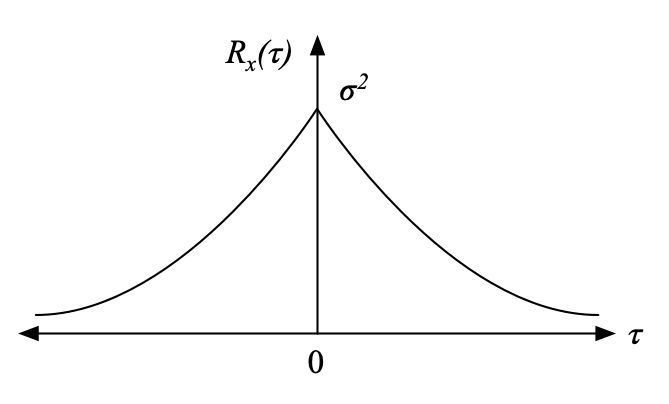
\includegraphics[width=\textwidth]{GM-Autocorrelation.png}
        \caption{Autocorrelation}
    \end{subfigure}
    \begin{subfigure}{0.49\textwidth}
        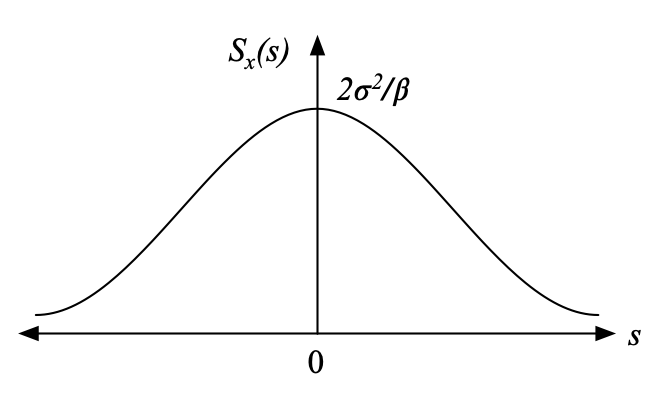
\includegraphics[width=\textwidth]{GM-Spectral-Density.png}
        \caption{Spectral Density}
    \end{subfigure}
    \caption{Gauss-Markov Autocorrelation and Spectral Density Functions}
    \label{fig:GM-characteristics}
\end{figure}

The Gauss-Markov process is a popular model because it seems to fit a large number of
physical processes, and because it is has a simple mathematical description. It basically
describes a process where its values are more correlated when the time spacing between
successive measurements is small, and less correlated when the time spacing between
successive measurements is large. It is a suitable model when nothing is known about the
underlying mechanics of the system state process and/or measurement acquisition process.

From linear system theory, we know that if we can factorize a spectral density function
into LHP and RHP forms of the same factor function $G(\cdot)$:

\begin{equation}
    S_x(s) = G(s) G(-s)
    \label{eq:Spectral-factorization}
\end{equation}

then $G(s)$ is the shaping filter that shapes unity white noise into the spectral density
$S_x(s)$. Thus, for the Gauss-Markov spectral density, we have

\begin{equation}
    S_x(s) = \left ( \frac{\sqrt{2 \sigma^2 \beta}}{s + \beta} \right ) \left ( \frac{\sqrt{2 \sigma^2 \beta}}{-s + \beta} \right )
    \label{eq:GM-spectral-factorization}
\end{equation}

and so the shaping filter is

\begin{equation}
    G(s) = \frac{\sqrt{2 \sigma^2 \beta}}{s + \beta}
    \label{eq:GM-shaping-filter}
\end{equation}

and the corresponding differential equation is

\begin{equation}
    \dot{x} = - \beta x + \sqrt{2 \sigma^2 \beta} \; w(t)
    \label{eq:GM-differential-equation}
\end{equation}

where $w(t)$ is a unity white noise process. Figure \ref{fig:GM-block-diagram} shows
the block diagram of the Gauss-Markov differential system.

\begin{figure}[ht]
    \centering
    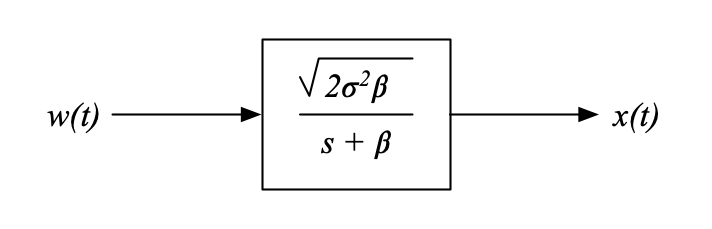
\includegraphics[width=0.5\textwidth]{GM-Block-Diagram.png}
    \caption{Gauss-Markov Process Block Diagram}
    \label{fig:GM-block-diagram}
\end{figure}

The complementary solution is

\begin{equation}
    x_c(t) = e^{-\beta t}
    \label{eq:GM-complementary-solution}
\end{equation}

Hence, the discrete-time state transition function is

\begin{equation}
    \phi_k = e^{-\beta \tau_k}
    \label{eq:GM-state-transition}
\end{equation}

and the discrete-time process variance is

\begin{equation}
    \setlength{\jot}{10pt}
    \begin{aligned}
    Q_k &= E[w_k^2] \\
        &= \int_0^{\tau_k} \left ( \sqrt{2 \sigma^2 \beta} \; e^{- \beta v} \right ) ^ 2 dv \\
        &= \sigma^2 \left ( 1 - e^{-2 \beta \tau_k} \right )
    \end{aligned}
    \label{eq:GM-process-variance}
\end{equation}

where $\tau_k = t_k - t_{k-1}$ represents the difference between two sample points in time
denoted by $k$ and $k - 1$.

The scalar discrete-time representation of the Gauss-Markov system is then

\begin{equation}
    x_k = \phi_k x_{k-1} + w_k
    \label{eq:GM-discrete-state-equation}
\end{equation}

\begin{equation}
    z_k = x_{k} + v_k
    \label{eq:GM-discrete-measurement-equation}
\end{equation}

where $z_k$ is the process measurement at the $k$th time point, $w_k$ is a white noise
sequence representing process noise with known variance

\begin{equation}
    E[w_k^2] = Q_k
    \label{eq:GM-discrete-process-variance}
\end{equation}

and where $v_k$ is a white noise sequence representing measurement error with known
variance

\begin{equation}
    E[v_k^2] = R_k
    \label{eq:GM-discrete-measurement-variance}
\end{equation}



%-------------------------------------------------------------------------------
%
% Gauss-Markov Kalman Filter
%
%-------------------------------------------------------------------------------

\clearpage
\section{Gauss-Markov Kalman Filter}

The Kalman filter implementation of a Gauss-Markov process model can be implemented
very efficiently since it involves only scalar arithmetic.

At the $k$th time point, we obtain a measurement $z_k$ at time $t_k$. We model our
measurement error with a variance $R_k$. At each time point, the filter provides a best
estimate, $\hat{x}_k$ and maintains a state estimate variance, $P_k$. We initialize the
filter with $\hat{x}_0 = z_0$ and $P_0 = P0$, where $P0$ is a suitably chosen value based
on empirical analysis.

For each acquisition event, $k$, we perform the following steps

1. Compute $\phi_k$ using (\ref{eq:GM-state-transition})

2. Compute $Q_k$ using (\ref{eq:GM-process-variance})

3. Compute state estimate prediction:

\begin{equation}
    \hat{x}_k^- = \phi_k \, \hat{x}_{k-1}
    \label{eq:GM-KF-x-prediction}
\end{equation}

4. Compute state estimate variance prediction:

\begin{equation}
    P_k^- = \phi_k \, P_{k-1} \, \phi_k + Q_k
    \label{eq:GM-KF-P-prediction}
\end{equation}

5. Compute Kalman gain:

\begin{equation}
    K_k = \frac{P_k^-}{P_k^- + R_k}
    \label{eq:GM-KF-gain}
\end{equation}

6. Compute state estimate correction:

\begin{equation}
    \hat{x}_k^+ = \hat{x}_k^- + K_k \,(z_k - \hat{x}_k^-)
    \label{eq:GM-KF-x-correction}
\end{equation}

7. Compute state estimate variance correction:

\begin{equation}
    P_k^+ = (1 - K_k) \, P_k^-
    \label{eq:GM-KF-P-correction}
\end{equation}



%-------------------------------------------------------------------------------
%
% Experiments
%
%-------------------------------------------------------------------------------

\clearpage
\section{Experiments}

A simple iOS application was developed that enables an iPhone to continuously scan for
nearby Bluetooth devices, reading among other properties, their RSSI, UUID, and device
name properties. Each reading gets timestamped and logged to a file that an be copied to
a computer for further processing. A simple Python script was written to selectively
filter and plot device data based on device UUID. The filter was a scalar Kalman filter
using a Gauss-Markov process as the model.

Two experiments were performed. The first experiment involved walking the scanning
iPhone (an iPhone Xs Max) away throughout the house (hallway and then dining room) from
the development MacBook Pro computer (kitchen) and then moved back again. The second
experiment involved taking both the scanning iPhone and a second iPhone outside and then
walking the scanning iPhone from the corner of the back yard to the second iPhone and then
away again. Figure \ref{fig:experiment-diagram} depicts a simple diagram of the walking
routes taken (shown in red) for each experiment. The distance values are approximate.

\begin{figure}[ht]
    \centering
    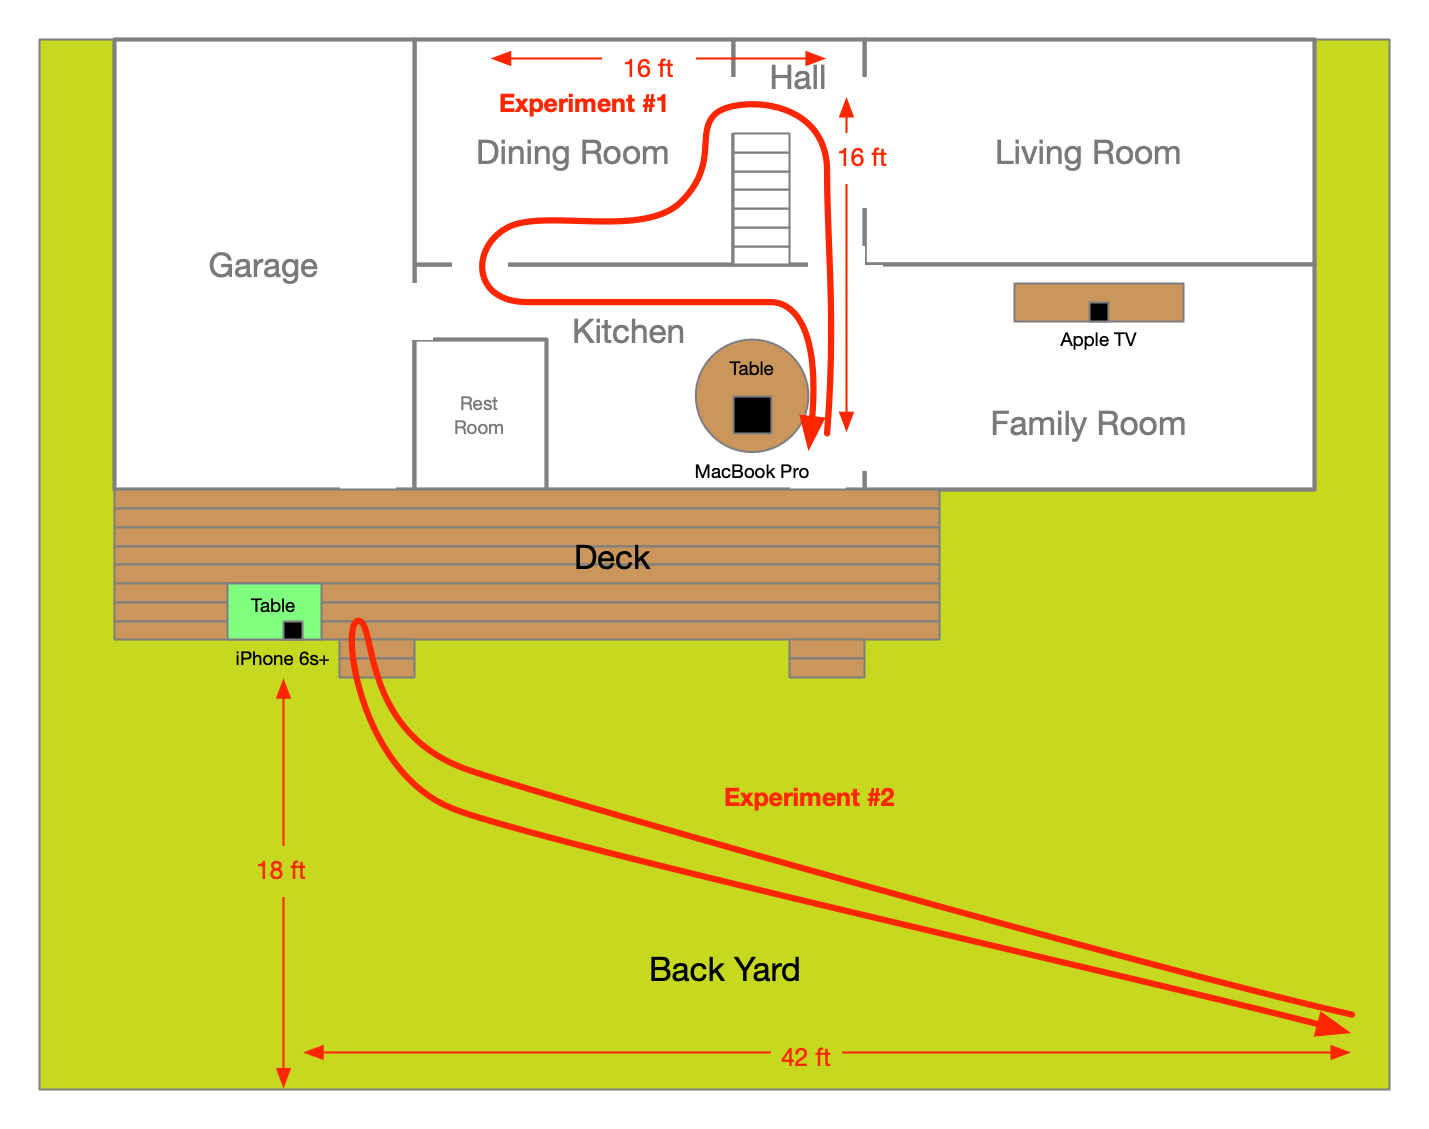
\includegraphics[width=1.0\textwidth]{RSSI-Experiment-Routes.png}
    \caption{Diagram of Experiment Walk Routes (Shown in Red)}
    \label{fig:experiment-diagram}
\end{figure}

One particular note about the second experiment was that the second iPhone screen was
active when the device was placed on a table on the deck before initiating the experiment,
but, by the time the walk from the corner of the yard had reached the second iPhone, it was
observed that the screen of the second iPhone had just gone to sleep. This can be seen in
the rate of the acquired data, where the "awake" condition produced more Bluetooth scan
responses than the "sleep" condition. This was a fortunate event, because it provided a
perfect data set to illustrate why a Gauss-Markov process model is suitable.

The Gauss-Markov Kalman filter was initialized with the following parameters:

\begin{center}
    \begin{tabular}{cccc}
        $P_0 = 5$ ,
        &
        $\sigma = 10$ ,
        &
        $\beta = 0.01$ ,
        &
        $R = 25$
    \end{tabular}
\end{center}

For the first experiment, the UUID of the development MacBook Pro (Red Green) was
monitored. The scanning iPhone was walked away from and then back to the computer. The
results can be seen in Figure \ref{fig:experiment-1-mbp}. The RSSI measurements are blue,
and the filtered RSSI values are in red.

\begin{figure}[ht]
    \centering
    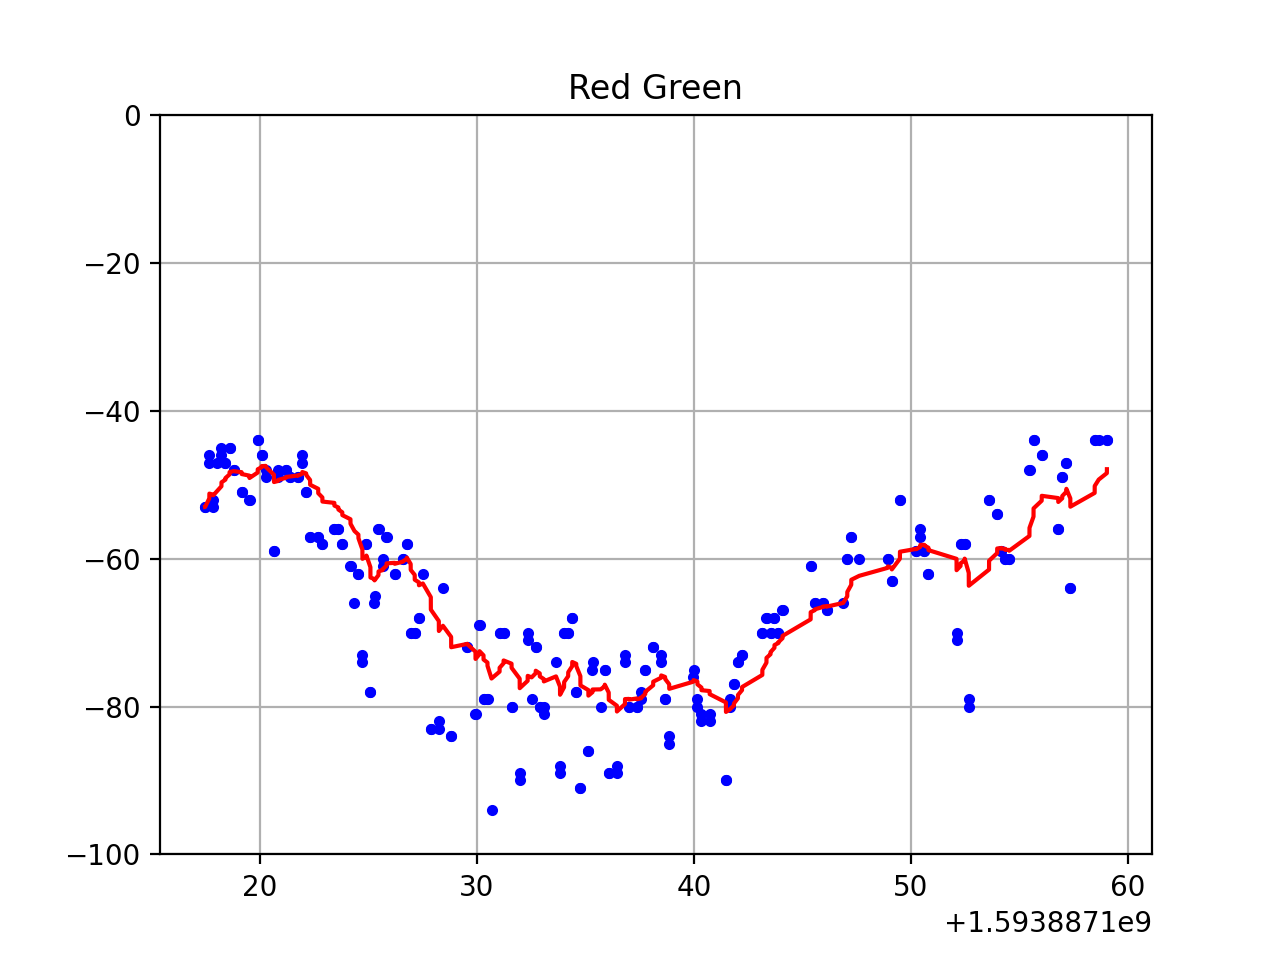
\includegraphics[width=1.0\textwidth]{Experiment-1-MBP-GM.png}
    \caption{Experiment \#1 - Scanning MacBook Pro from Indoors}
    \label{fig:experiment-1-mbp}
\end{figure}

For the second experiment, both the scanning iPhone and the second stationary iPhone
(an iPhone 6s+) were outside in the back yard. The scanning iPhone was walked from the
corner of the yard to the stationary iPhone and back again. As was stated previously,
the stationary iPhone screen went to sleep when the scanning iPhone reached the stationary
iPhone location. The scanning iPhone was then walked away back to the corner of the yard.
The results for the second iPhone can be seen in Figure \ref{fig:experiment-2-iphone}.

\begin{figure}[ht]
    \centering
    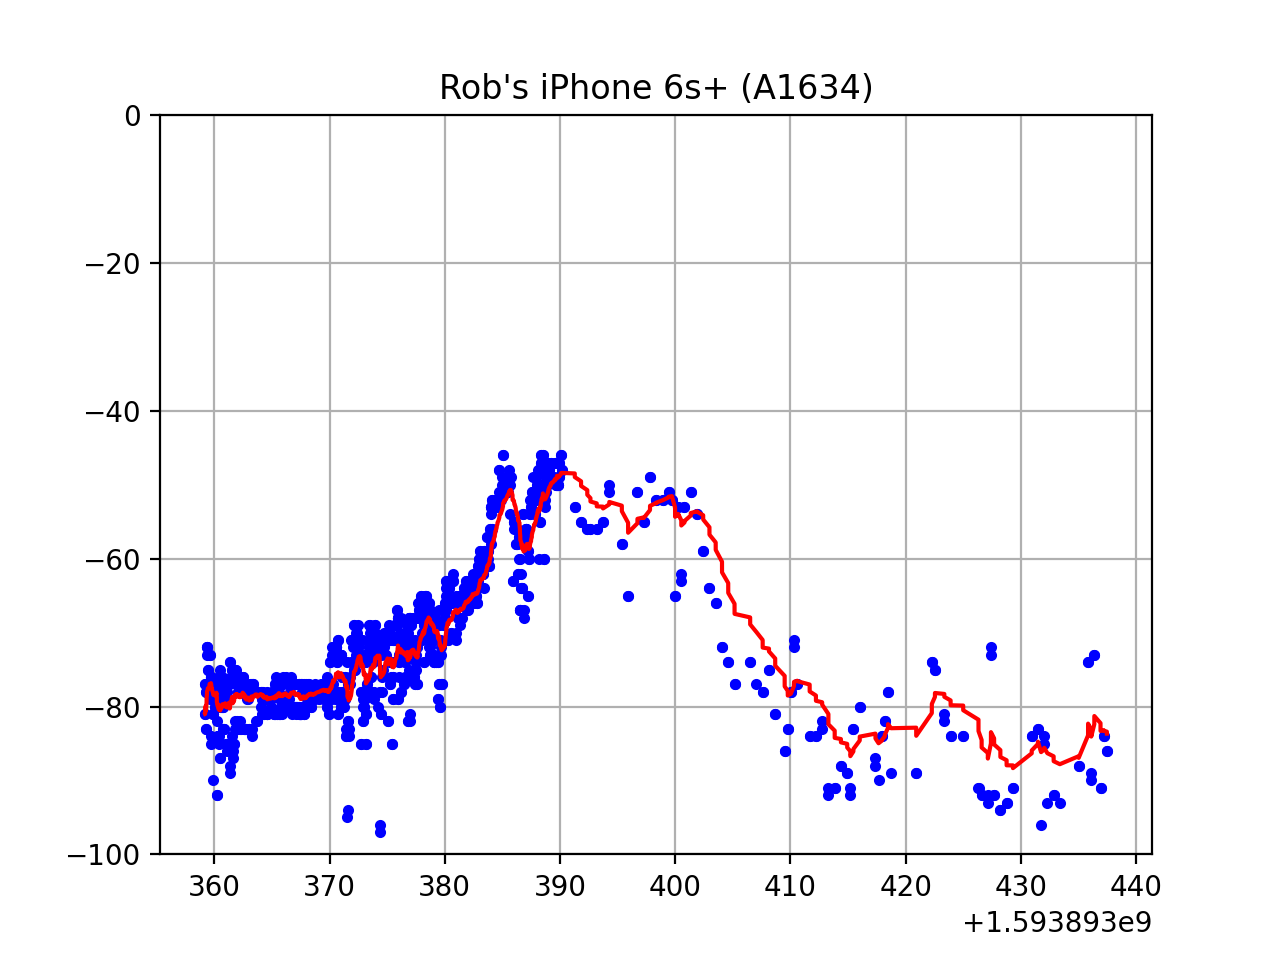
\includegraphics[width=1.0\textwidth]{Experiment-2-iPhone-GM.png}
    \caption{Experiment \#2 - Scanning Second iPhone from Back Yard}
    \label{fig:experiment-2-iphone}
\end{figure}

Also available from the second experiment was the scanned Bluetooth signal data from both
the development MacBook Pro computer in the kitchen, and an Apple TV in the family room.
As shown in Figure \ref{fig:experiment-diagram}, both devices are in rooms that face the
back yard, and their distances from the scanning iPhone are comparable. The results for
the MacBook Pro can be seen in Figure \ref{fig:experiment-2-mbp}, and the results for the
Apple TV can be seen in Figure \ref{fig:experiment-2-atv}.

\begin{figure}[ht]
    \centering
    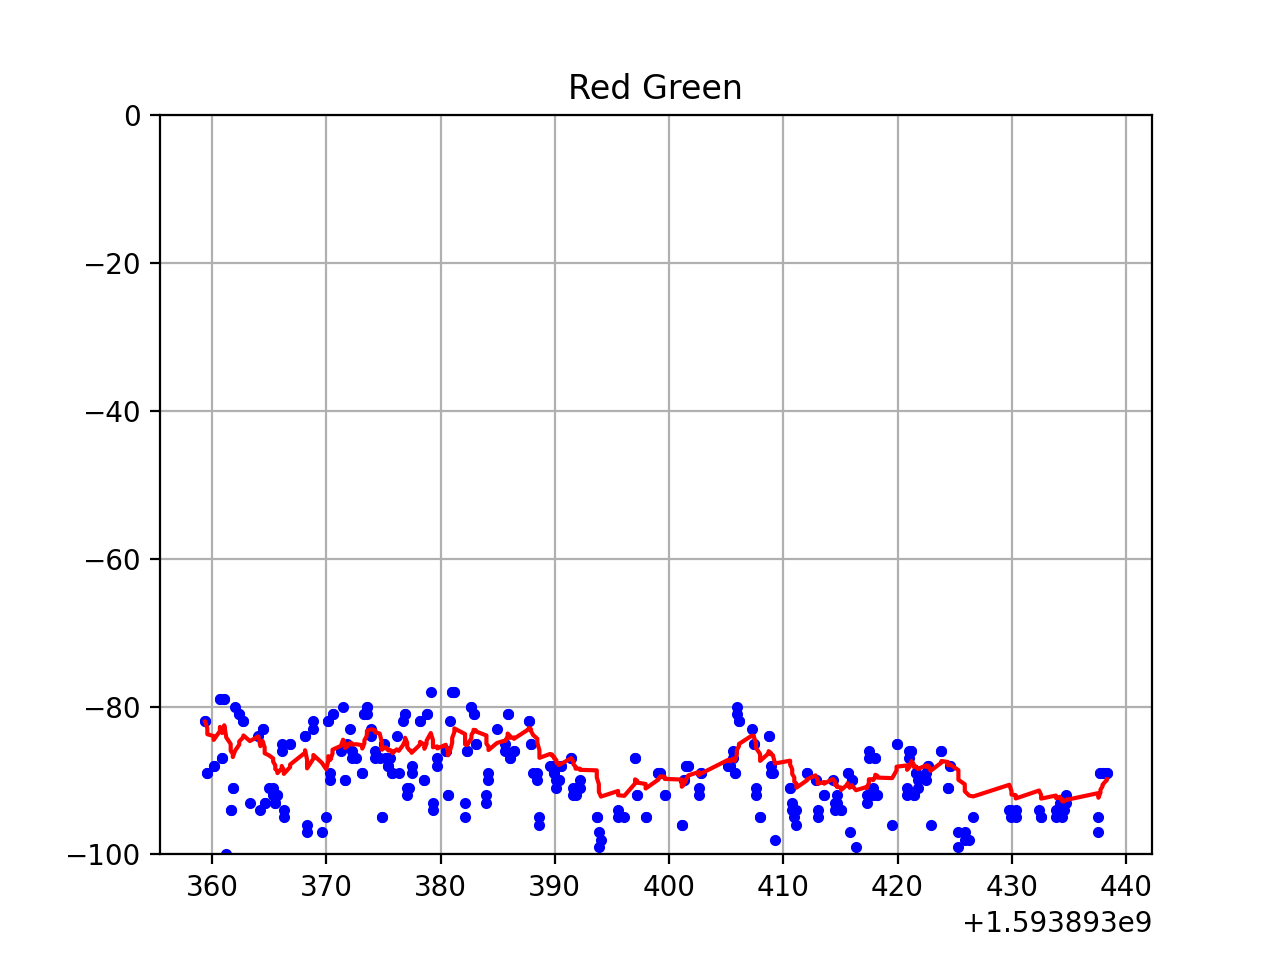
\includegraphics[width=1.0\textwidth]{Experiment-2-MBP-GM.png}
    \caption{Experiment \#2 - Scanning MacBook Pro from Back Yard}
    \label{fig:experiment-2-mbp}
\end{figure}

\begin{figure}[ht]
    \centering
    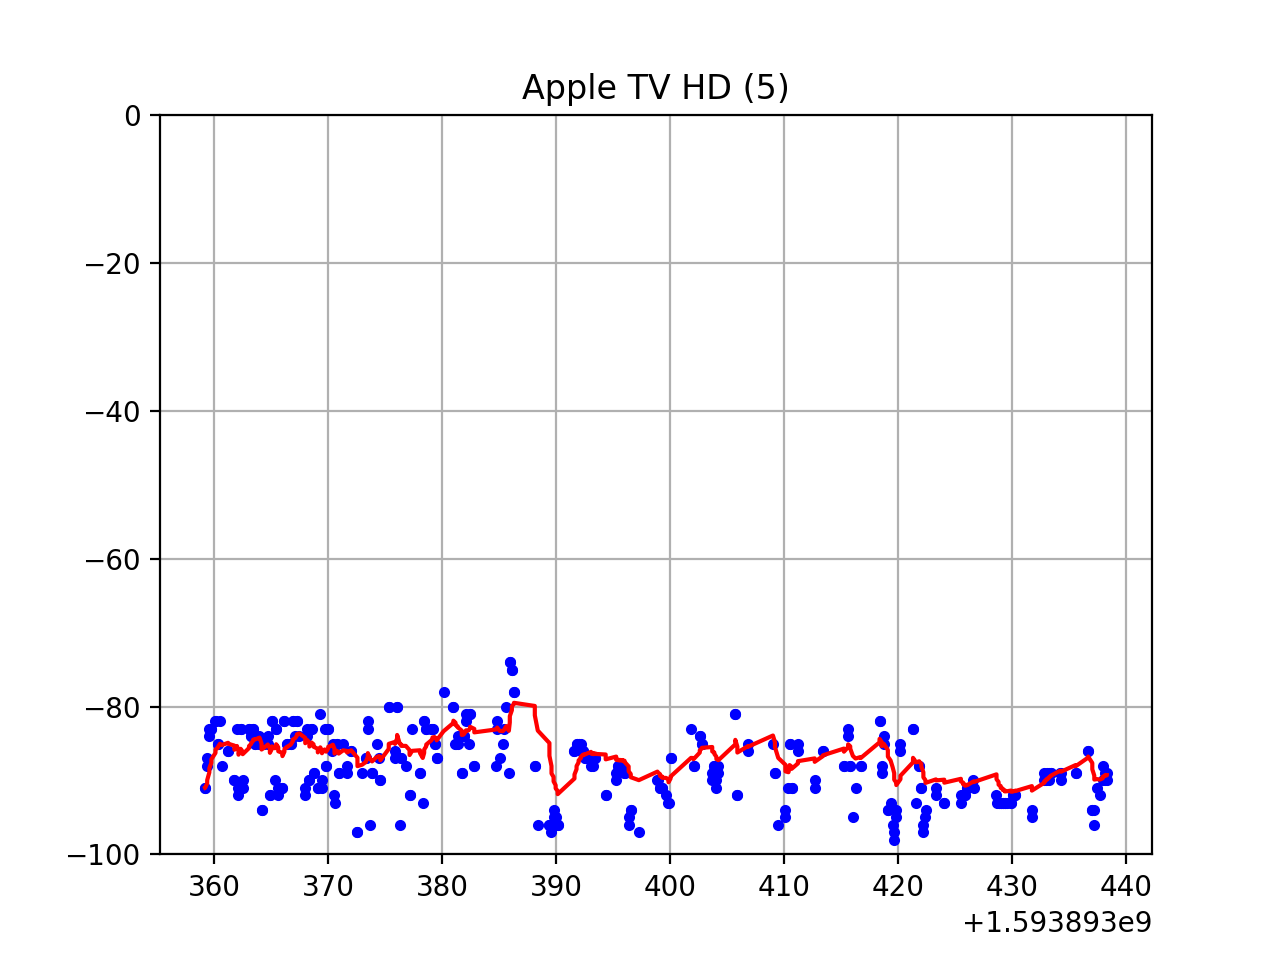
\includegraphics[width=1.0\textwidth]{Experiment-2-ATV-GM.png}
    \caption{Experiment \#2 - Scanning Apple TV from Back Yard}
    \label{fig:experiment-2-atv}
\end{figure}



%-------------------------------------------------------------------------------
%
% Gauss-Markov Process with Random Bias
%
%-------------------------------------------------------------------------------

\clearpage
\section{Gauss-Markov Process with Random Bias}

The Gauss-Markov process can be augmented with a random bias process to model certain
systems that seem to have a Gauss-Markov behavior offset by a random bias \cite{rgbrown1983}.
The model differential equations are

\begin{equation}
    \begin{bmatrix}
    \dot{x_1} \\
    \phantom{m} \\
    \dot{x_2}
    \end{bmatrix}
    =
    \begin{bmatrix}
    0 & & 0 \\
    \phantom{m} \\
    0 & & -\beta_g
    \end{bmatrix}
    \begin{bmatrix}
    x_1 \\
    \phantom{m} \\
    x_2
    \end{bmatrix}
    +
    \begin{bmatrix}
    1 & & 0 \\
    \phantom{m} \\
    0 & & \sqrt{2 \sigma_g^2 \beta_g}
    \end{bmatrix}
    \begin{bmatrix}
    w_b \\
    \phantom{m} \\
    w_g
    \end{bmatrix}
    \label{eq:GMRB-differential-system}
\end{equation}

\begin{equation}
    y = 
    \begin{bmatrix}
    1 & & 1
    \end{bmatrix}
    \begin{bmatrix}
    x_1 \\
    \phantom{m} \\
    x_2
    \end{bmatrix}
    +
    v
    \label{eq:GMRB-observation}
\end{equation}

where $v$ is the measurement-error zero-mean Gaussian random process.

Figure \ref{fig:GMRB-block-diagram} illustrates the block diagram for the Gauss-Markov
process with random bias.

\begin{figure}[ht]
    \centering
    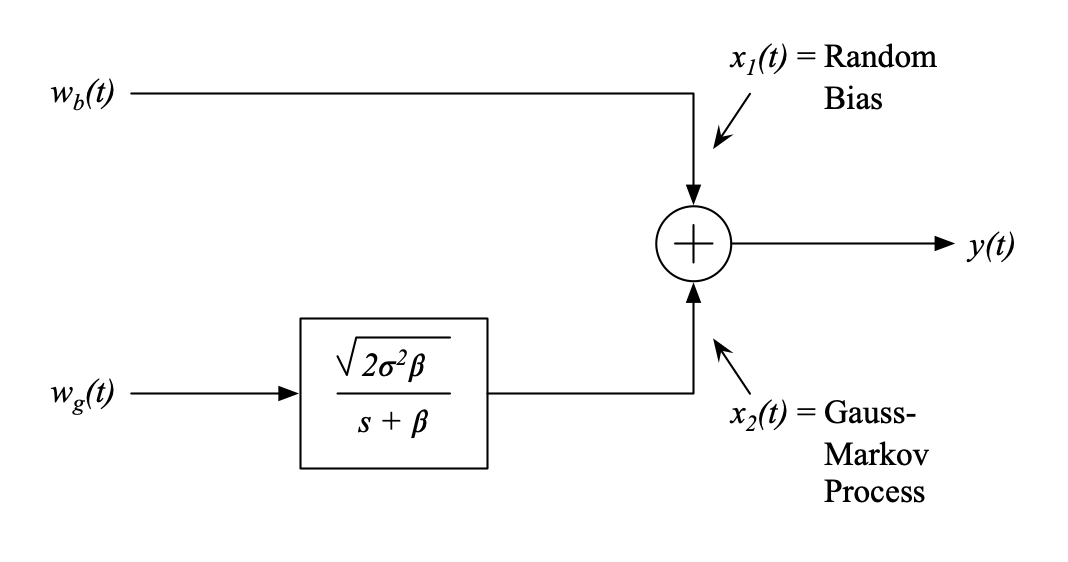
\includegraphics[width=0.8\textwidth]{GMRB-Block-Diagram.png}
    \caption{Gauss-Markov with Random Bias Block Diagram}
    \label{fig:GMRB-block-diagram}
\end{figure}

The vector discrete-time representation of the Gauss-Markov with random bias is

\begin{equation}
    \mathbf{x}_k = \mathbf{\Phi}_k \mathbf{x}_{k-1} + \mathbf{w}_k
    \label{eq:GMRB-discrete-state-equation}
\end{equation}

\begin{equation}
    \mathbf{z}_k = \mathbf{H}_k \mathbf{x}_{k} + \mathbf{v}_k
    \label{eq:GMRB-discrete-measurement-equation}
\end{equation}

where $\mathbf{w}_k$ is a white noise sequence representing process noise with known
covariance

\begin{equation}
    E[\mathbf{w}_k \mathbf{w}_k^T] = \mathbf{Q}_k
    \label{eq:GMRB-discrete-process-covariance}
\end{equation}

and where $\mathbf{v}_k$ is a white noise sequence representing measurement error with
known measurement error covariance

\begin{equation}
    E[\mathbf{v}_k \mathbf{v}_k^T] = \mathbf{R}_k
    \label{eq:GMRB-discrete-measurement-covariance}
\end{equation}

In order to specify the discrete-time matrix values, as before we define the discrete-time
difference to be $\tau_k = t_k - t_{k-1}$.

The discrete-time state transition matrix is

\begin{equation}
    \mathbf{\Phi}_k = 
    \begin{bmatrix}
    1  & \phantom{m} &  0 \\
    \phantom{m} \\
    0  & \phantom{m} &  e^{- \beta_g \tau_k}
    \end{bmatrix}
    \label{eq:GMRB-state-transition}
\end{equation}

The process covariance matrix is

\begin{equation}
    \mathbf{Q}_k = 
    \begin{bmatrix}
    \sigma_b^2  & \phantom{m} &  0 \\
    \phantom{m} \\
    0  & \phantom{m} &  \sigma_g^2 \left ( 1 - e^{-2 \beta_g \tau_k} \right )
    \end{bmatrix}
    \label{eq:GMRB-process-Q}
\end{equation}

where $\sigma_b^2$ is the mean-square value of the random bias, $\sigma_g^2$ is the
Gauss-Markov process mean-square value, and $1 / \beta_g$ is the Gauss-Markov process
time constant.

Lastly, the measurement transformation matrix is

\begin{equation}
    \mathbf{H}_k = 
    \begin{bmatrix}
    1  & &  1
    \end{bmatrix}
    \label{eq:GMRB-measurement-H}
\end{equation}



%-------------------------------------------------------------------------------
%
% Gauss-Markov with Random Bias Kalman Filter
%
%-------------------------------------------------------------------------------

\clearpage
\section{Gauss-Markov with Random Bias Kalman Filter}

The Kalman filter implementation of a Gauss-Markov with random bias process model can be
implemented efficiently since it involves only $2 \times 2$ matrix arithmetic.

At the $k$th time point, we obtain a measurement $\mathbf{z}_k$ at time $t_k$. We model
our measurement error with a covariance $\mathbf{R}_k$. At each time point, the filter
provides a best estimate, $\hat{\mathbf{x}}_k$ and maintains a state estimate covariance,
$\mathbf{P}_k$. We initialize the filter with $\hat{\mathbf{x}}_0 = \mathbf{z}_0$ and
$\mathbf{P}_0 = \mathbf{P0}$, where $\mathbf{P0}$ is a suitably chosen value based on empirical
analysis.

For each acquisition event, $k$, we perform the following steps

1. Compute $\mathbf{\Phi}_k$ using (\ref{eq:GMRB-state-transition})

2. Compute $\mathbf{Q}_k$ using (\ref{eq:GMRB-process-Q})

3. Compute state estimate prediction:

\begin{equation}
    \hat{\mathbf{x}}_k^- = \mathbf{\Phi}_k \hat{\mathbf{x}}_{k-1}
    \label{eq:GMRB-KF-x-prediction}
\end{equation}

4. Compute state estimate variance prediction:

\begin{equation}
    \mathbf{P}_k^- = \mathbf{\Phi}_k \mathbf{P}_k \mathbf{\Phi}_k^T + \mathbf{Q}_k
    \label{eq:GMRB-KF-P-prediction}
\end{equation}

5. Compute Kalman gain:

\begin{equation}
    \mathbf{K}_k = \mathbf{P}_k^- \mathbf{H}_k^T
        \left (
            \mathbf{H}_k \mathbf{P}_k^- \mathbf{H}_k^T + \mathbf{R}_k
        \right )^{-1}
    \label{eq:GMRB-KF-gain}
\end{equation}

6. Compute state estimate correction:

\begin{equation}
    \hat{\mathbf{x}}_k^+ = \hat{\mathbf{x}}_k^- + \mathbf{K}_k
    \left (
        \mathbf{z}_k - \mathbf{H}_k \hat{\mathbf{x}}_k^-
    \right )
    \label{eq:GMRB-KF-x-correction}
\end{equation}

7. Compute state estimate variance correction:

\begin{equation}
    \mathbf{P}_k^+ = \left ( \mathbf{I} - \mathbf{K}_k \mathbf{H}_k \right ) \mathbf{P}_k^-
    \label{eq:GMRB-KF-P-correction}
\end{equation}



%-------------------------------------------------------------------------------
%
% Experiments - Gauss-Markov with Random Bias
%
%-------------------------------------------------------------------------------

\clearpage
\section{Experiments - Gauss-Markov with Random Bias}

Using the data from our previous experiments, we can evaluate the Kalman filter using the
Gauss-Markov with random bias model. Our Kalman filter was initialized with the following
parameters:

\begin{center}
    \begin{tabular}{cccc}
        $\mathbf{P}_0 = 
        \begin{bmatrix}
        5 & 0 \\
        0  & 5
        \end{bmatrix}$ ,
        &
        $\sigma_b = 0.5$ ,
        &
        $\begin{aligned}
        \sigma_g &= 1 \\
        \beta_g  &= 0.1
        \end{aligned}$ ,
        &
        $R = 25$
    \end{tabular}
\end{center}

Using the Gauss-Markov with Random Bias model on the data of the first experiment for
the UUID of the MacBook Pro computer produces the results shown in Figure
\ref{fig:experiment-1-mbp-gmrb}. As before, the RSSI measurements are blue, and the
filtered RSSI values are in red.

\begin{figure}[ht]
    \centering
    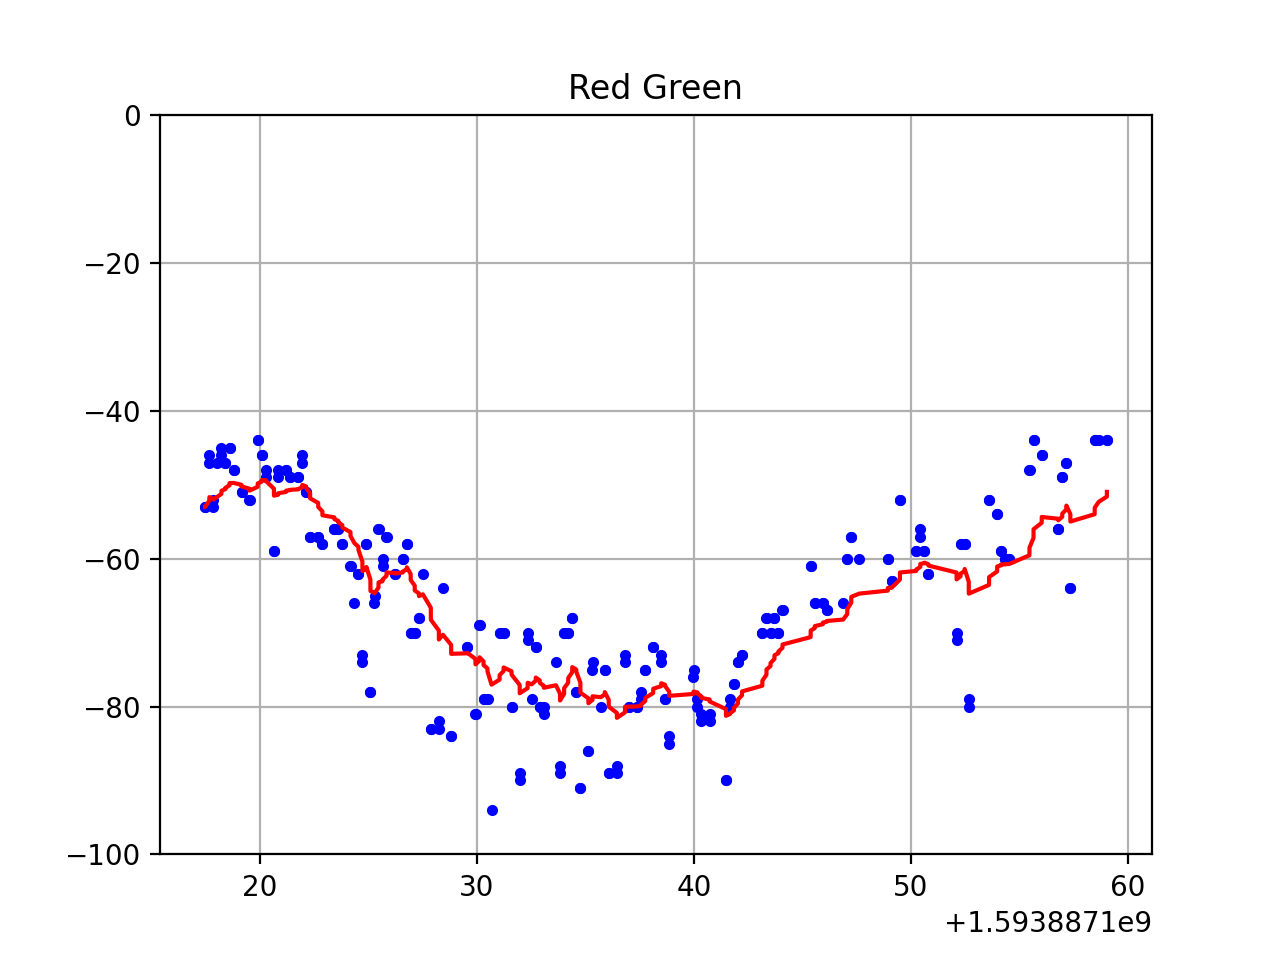
\includegraphics[width=1.0\textwidth]{Experiment-1-MBP-GMRB.png}
    \caption{Experiment \#1 - MacBook Pro, Gauss-Markov with Random Bias}
    \label{fig:experiment-1-mbp-gmrb}
\end{figure}

Using the Gauss-Markov with Random Bias model on the data of the second experiment for
the UUID of the stationary iPhone produces the results shown in Figure
\ref{fig:experiment-2-iphone-gmrb}.

\begin{figure}[ht]
    \centering
    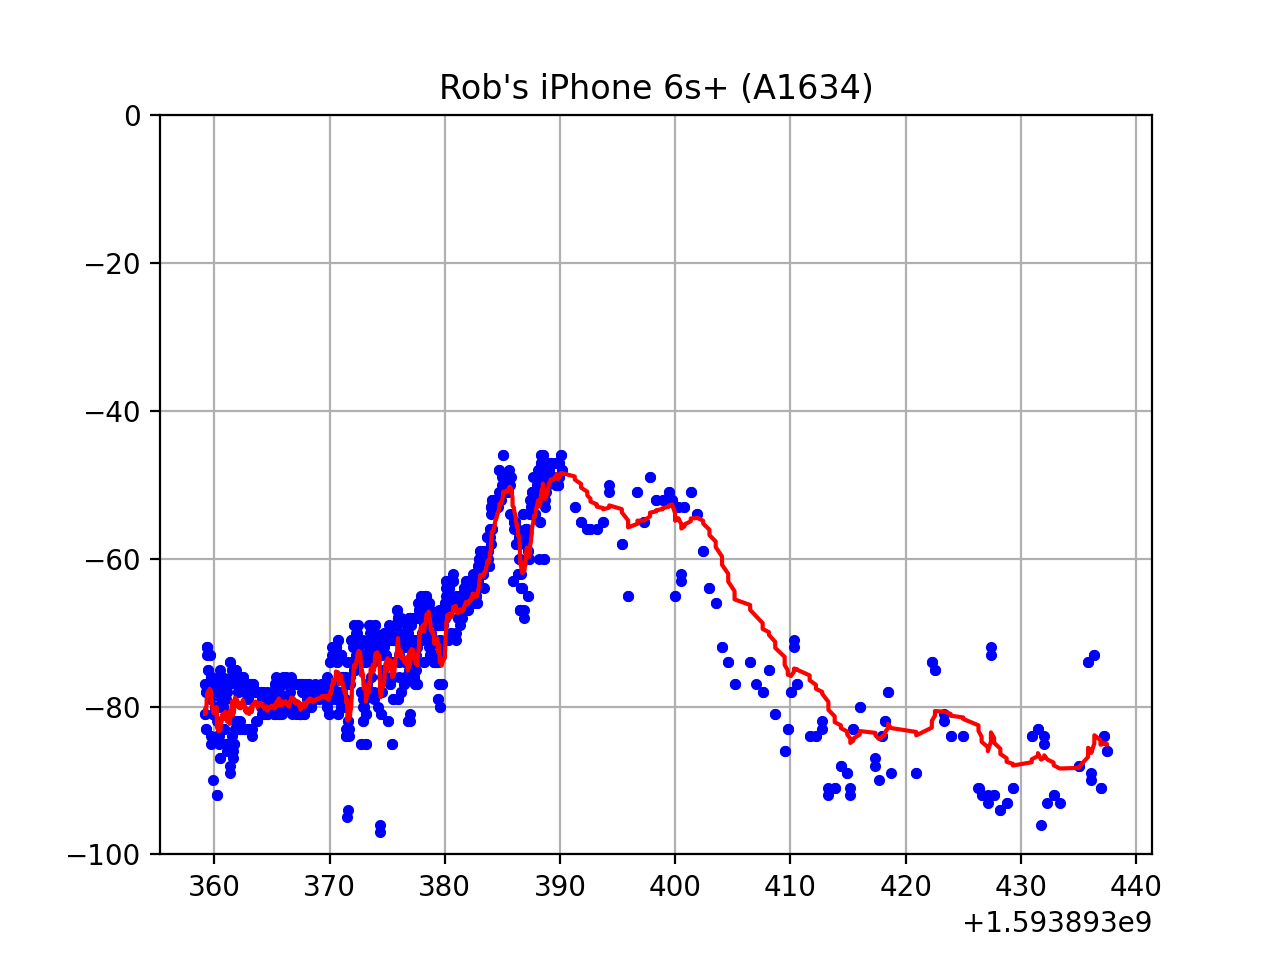
\includegraphics[width=1.0\textwidth]{Experiment-2-iPhone-GMRB.png}
    \caption{Experiment \#2 - iPhone, Gauss-Markov with Random Bias}
    \label{fig:experiment-2-iphone-gmrb}
\end{figure}

It does not appear that the Gauss-Markov with random bias model offers a noticeable
improvement over the Gauss-Markov model. Given the added processing complexity in going
from a scalar filer to a $2 \times 2$ matrix filter, this filter model is not a viable
choice for this particular application.

For completeness, the back yard results for the MacBook Pro can be seen in Figure
\ref{fig:experiment-2-mbp-gmrb}, and the results for the Apple TV can be seen in Figure
\ref{fig:experiment-2-atv-gmrb}.

\begin{figure}[ht]
    \centering
    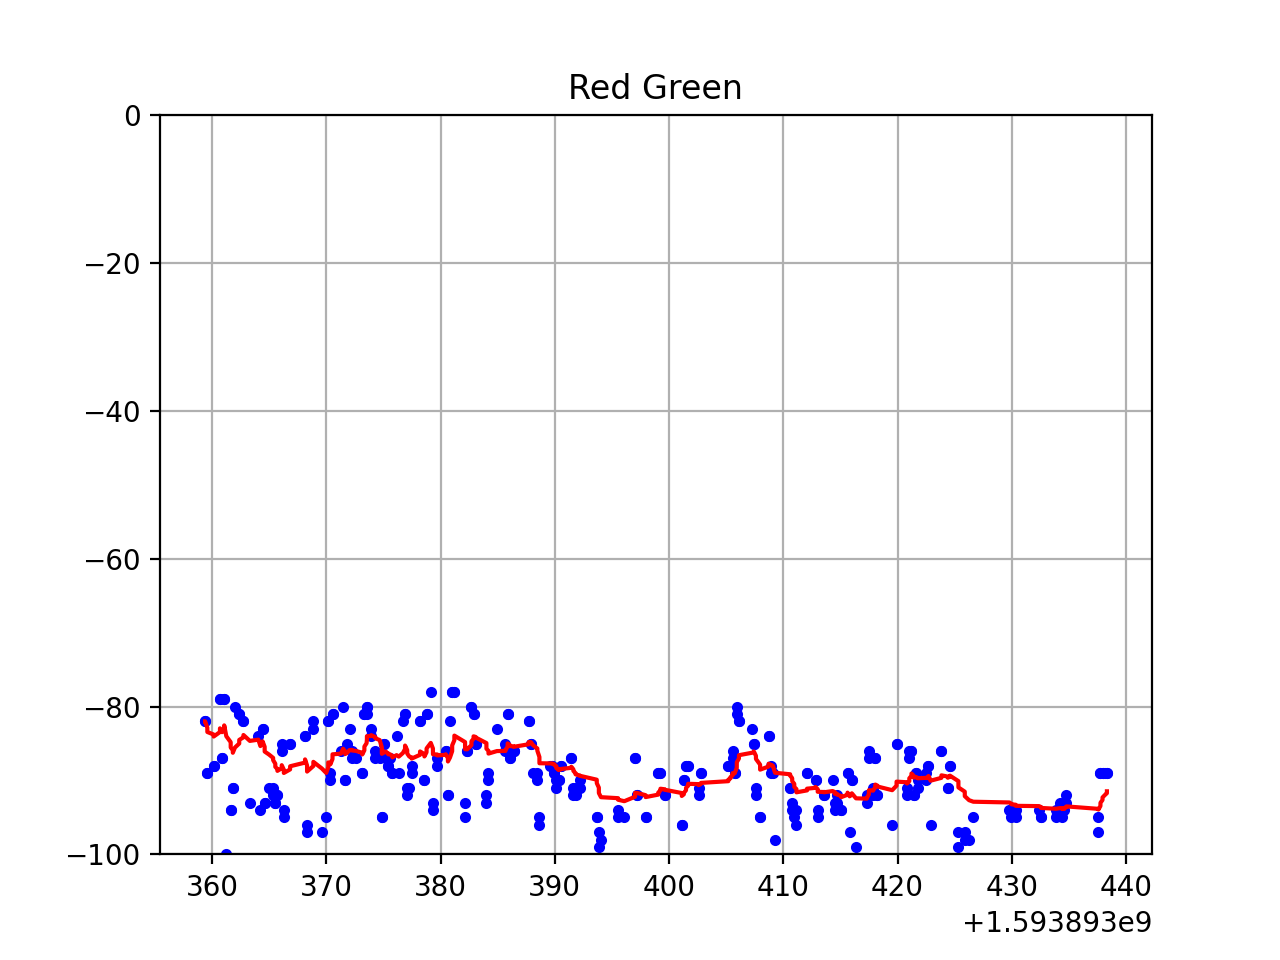
\includegraphics[width=1.0\textwidth]{Experiment-2-MBP-GMRB.png}
    \caption{Experiment \#2 - MacBook Pro, Gauss-Markov with Random Bias}
    \label{fig:experiment-2-mbp-gmrb}
\end{figure}

\begin{figure}[ht]
    \centering
    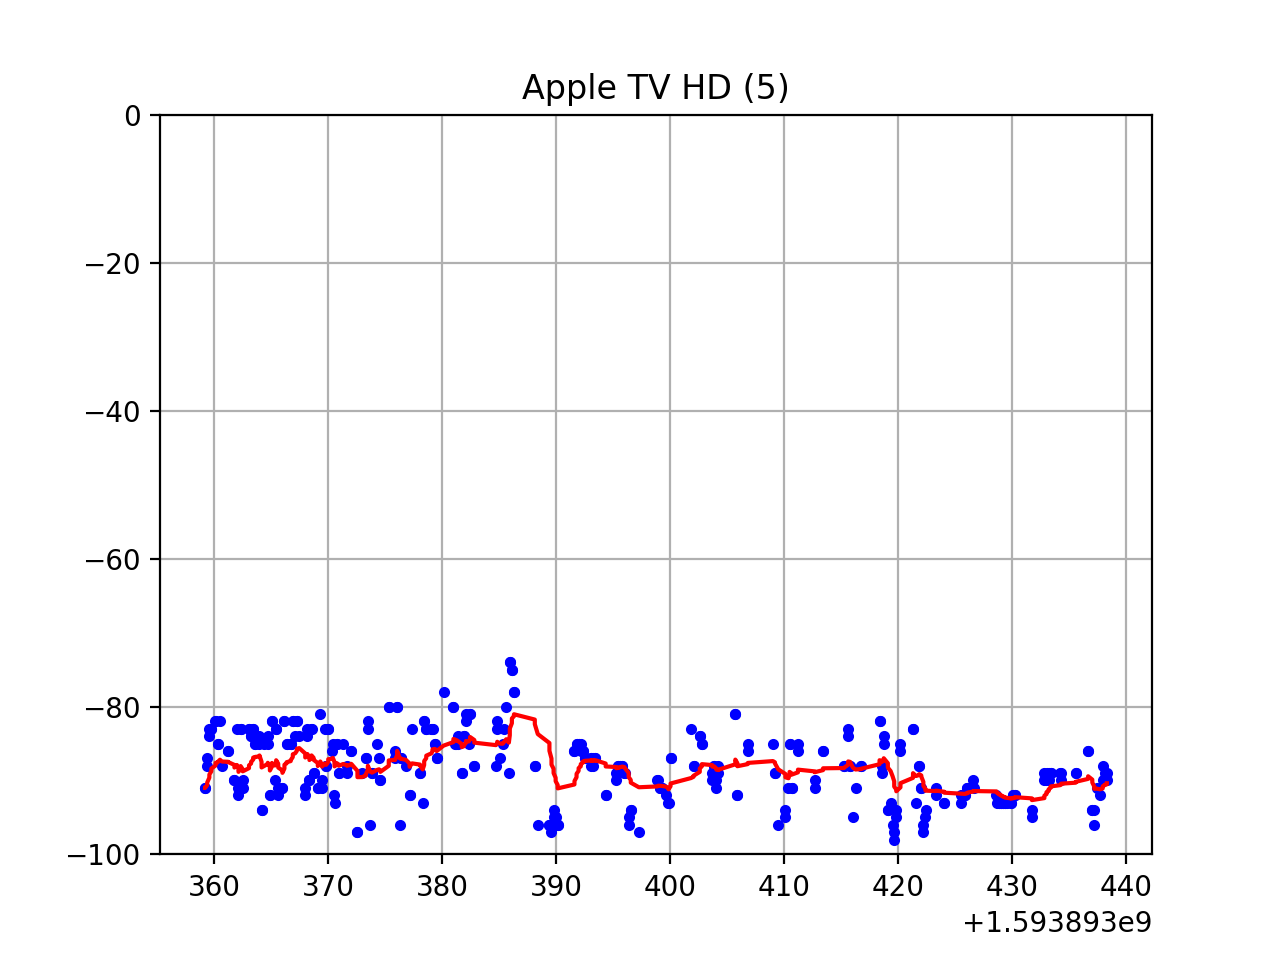
\includegraphics[width=1.0\textwidth]{Experiment-2-ATV-GMRB.png}
    \caption{Experiment \#2 - Apple TV, Gauss-Markov with Random Bias}
    \label{fig:experiment-2-atv-gmrb}
\end{figure}



%-------------------------------------------------------------------------------
%
% Integrated Gauss-Markov Process
%
%-------------------------------------------------------------------------------

\clearpage
\section{Integrated Gauss-Markov Process}

A useful process model based on the Gauss-Markov process is the integrated Gauss-Markov
process \cite{rgbrown1983}. This model is a popular model used in many engineering
applications because it characterizes a low-pass filtered Gauss-Markov process. The model
differential equations are

\begin{equation}
    \begin{bmatrix}
    \dot{x_1} \\
    \phantom{m} \\
    \dot{x_2}
    \end{bmatrix}
    =
    \begin{bmatrix}
    0 & & 1 \\
    \phantom{m} \\
    0 & & -\beta
    \end{bmatrix}
    \begin{bmatrix}
    x_1 \\
    \phantom{m} \\
    x_2
    \end{bmatrix}
    +
    \begin{bmatrix}
    0 \\
    \phantom{m} \\
    \sqrt{2 \sigma^2 \beta}
    \end{bmatrix}
    w
    \label{eq:IGM-differential-system}
\end{equation}

\begin{equation}
    y = 
    \begin{bmatrix}
    1 & & 0
    \end{bmatrix}
    \begin{bmatrix}
    x_1 \\
    \phantom{m} \\
    x_2
    \end{bmatrix}
    +
    v
    \label{eq:IGM-observation}
\end{equation}

where $v$ is the measurement-error zero-mean Gaussian random process.

Figure \ref{fig:IGM-block-diagram} shows the block diagram of the integrated Gauss-Markov
differential system.

\begin{figure}[ht]
    \centering
    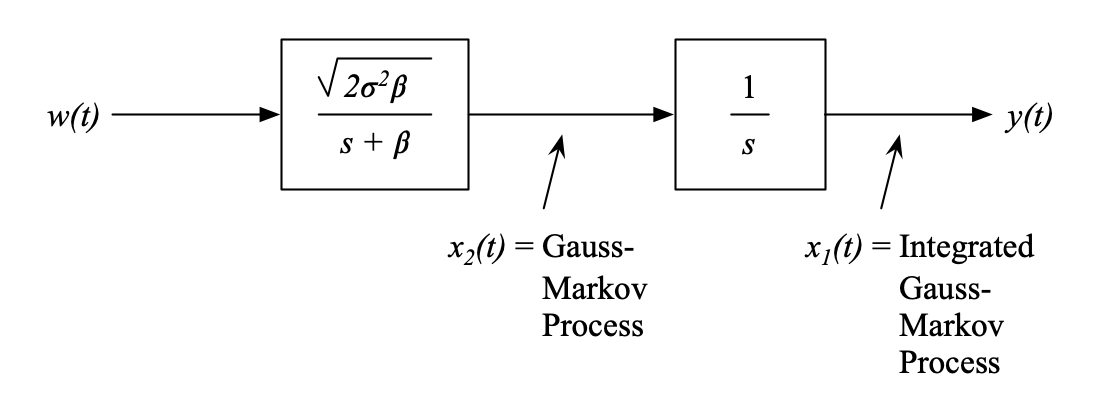
\includegraphics[width=0.8\textwidth]{IGM-Block-Diagram.png}
    \caption{Integrated Gauss-Markov Process Block Diagram}
    \label{fig:IGM-block-diagram}
\end{figure}

The vector discrete-time representation of integrated Gauss-Markov system is

\begin{equation}
    \mathbf{x}_k = \mathbf{\Phi}_k \mathbf{x}_{k-1} + \mathbf{w}_k
    \label{eq:IGM-discrete-state-equation}
\end{equation}

\begin{equation}
    \mathbf{z}_k = \mathbf{H}_k \mathbf{x}_{k} + \mathbf{v}_k
    \label{eq:IGM-discrete-measurement-equation}
\end{equation}

where $\mathbf{w}_k$ is a white noise sequence representing process noise with known
covariance

\begin{equation}
    E[\mathbf{w}_k \mathbf{w}_k^T] = \mathbf{Q}_k
    \label{eq:IGM-discrete-process-covariance}
\end{equation}

and where $\mathbf{v}_k$ is a white noise sequence representing measurement error with
known measurement error covariance

\begin{equation}
    E[\mathbf{v}_k \mathbf{v}_k^T] = \mathbf{R}_k
    \label{eq:IGM-discrete-measurement-covariance}
\end{equation}

In order to specify the discrete-time matrix values, as before we define the discrete-time
difference to be $\tau_k = t_k - t_{k-1}$.

The discrete-time state transition matrix is

\begin{equation}
    \mathbf{\Phi}_k = 
    \begin{bmatrix}
    1  & \phantom{m} &  \dfrac{1}{\beta} \left ( 1 - e^{- \beta \tau_k} \right ) \\
    \phantom{m} \\
    0  & \phantom{m} &  e^{- \beta \tau_k}
    \end{bmatrix}
    \label{eq:IGM-state-transition}
\end{equation}

The process mean-square values for the process covariance matrix are

\begin{equation}
    E[x_1 x_1] = \frac{2 \sigma^2}{\beta}
        \left [
            \tau_k - \frac{2}{\beta} \left ( 1 - e^{- \beta \tau_k} \right )
                   + \frac{1}{2 \beta} \left ( 1 - e^{-2 \beta \tau_k} \right )
        \right ]
    \label{eq:IGM-Ex1x1}
\end{equation}

\begin{equation}
    E[x_1 x_2] = 2 \sigma^2
        \left [
            \frac{1}{\beta} \left ( 1 - e^{- \beta \tau_k} \right )
            - \frac{1}{2 \beta} \left ( 1 - e^{-2 \beta \tau_k} \right )
        \right ]
    \label{eq:IGM-Ex1x2}
\end{equation}

\begin{equation}
    E[x_2 x_2] = \sigma^2 \left ( 1 - e^{-2 \beta \tau_k} \right )
    \label{eq:IGM-Ex2x2}
\end{equation}

and so the process covariance matrix is

\begin{equation}
    \mathbf{Q}_k = 
    \begin{bmatrix}
    E[x_1 x_1]  & \phantom{m} &  E[x_1 x_2] \\
    \phantom{m} \\
    E[x_1 x_2]  & \phantom{m} &  E[x_2 x_2]
    \end{bmatrix}
    \label{eq:IGM-process-Q}
\end{equation}

Lastly, the measurement transformation matrix is

\begin{equation}
    \mathbf{H}_k = 
    \begin{bmatrix}
    1  & &  0
    \end{bmatrix}
    \label{eq:IGM-measurement-H}
\end{equation}



%-------------------------------------------------------------------------------
%
% Integrated Gauss-Markov Kalman Filter
%
%-------------------------------------------------------------------------------

\clearpage
\section{Integrated Gauss-Markov Kalman Filter}

The Kalman filter implementation of an integrated Gauss-Markov process model can be
implemented efficiently since it involves only $2 \times 2$ matrix arithmetic.

At the $k$th time point, we obtain a measurement $\mathbf{z}_k$ at time $t_k$. We model
our measurement error with a covariance $\mathbf{R}_k$. At each time point, the filter
provides a best estimate, $\hat{\mathbf{x}}_k$ and maintains a state estimate covariance,
$\mathbf{P}_k$. We initialize the filter with $\hat{\mathbf{x}}_0 = \mathbf{z}_0$ and
$\mathbf{P}_0 = \mathbf{P0}$, where $\mathbf{P0}$ is a suitably chosen value based on
empirical analysis.

For each acquisition event, $k$, we perform the following steps

1. Compute $\mathbf{\Phi}_k$ using (\ref{eq:IGM-state-transition})

2. Compute $\mathbf{Q}_k$ using (\ref{eq:IGM-process-Q})

3. Compute state estimate prediction:

\begin{equation}
    \hat{\mathbf{x}}_k^- = \mathbf{\Phi}_k \hat{\mathbf{x}}_{k-1}
    \label{eq:IGM-KF-x-prediction}
\end{equation}

4. Compute state estimate variance prediction:

\begin{equation}
    \mathbf{P}_k^- = \mathbf{\Phi}_k \mathbf{P}_k \mathbf{\Phi}_k^T + \mathbf{Q}_k
    \label{eq:IGM-KF-P-prediction}
\end{equation}

5. Compute Kalman gain:

\begin{equation}
    \mathbf{K}_k = \mathbf{P}_k^- \mathbf{H}_k^T
        \left (
            \mathbf{H}_k \mathbf{P}_k^- \mathbf{H}_k^T + \mathbf{R}_k
        \right )^{-1}
    \label{eq:IGM-KF-gain}
\end{equation}

6. Compute state estimate correction:

\begin{equation}
    \hat{\mathbf{x}}_k^+ = \hat{\mathbf{x}}_k^- + \mathbf{K}_k
    \left (
        \mathbf{z}_k - \mathbf{H}_k \hat{\mathbf{x}}_k^-
    \right )
    \label{eq:IGM-KF-x-correction}
\end{equation}

7. Compute state estimate variance correction:

\begin{equation}
    \mathbf{P}_k^+ = \left ( \mathbf{I} - \mathbf{K}_k \mathbf{H}_k \right ) \mathbf{P}_k^-
    \label{eq:IGM-KF-P-correction}
\end{equation}



%-------------------------------------------------------------------------------
%
% Experiments - Integrated Gauss-Markov
%
%-------------------------------------------------------------------------------

\clearpage
\section{Experiments - Integrated Gauss-Markov Model}

Using the data from our previous experiments, we can evaluate the Kalman filter using the
integrated Gauss-Markov model. Our Kalman filter was initialized with the following
parameters:

\begin{center}
    \begin{tabular}{cccc}
        $\mathbf{P}_0 = \mathbf{I}$ ,
        &
        $\sigma = 0.2$ ,
        &
        $\beta = 0.1$ ,
        &
        $R = 25$
    \end{tabular}
\end{center}

Using the integrated Gauss-Markov model on the data of the first experiment for
the UUID of the MacBook Pro computer produces the results shown in Figure
\ref{fig:experiment-1-mbp-igm}. As before, the RSSI measurements are blue, and the
filtered RSSI values are in red.

\begin{figure}[ht]
    \centering
    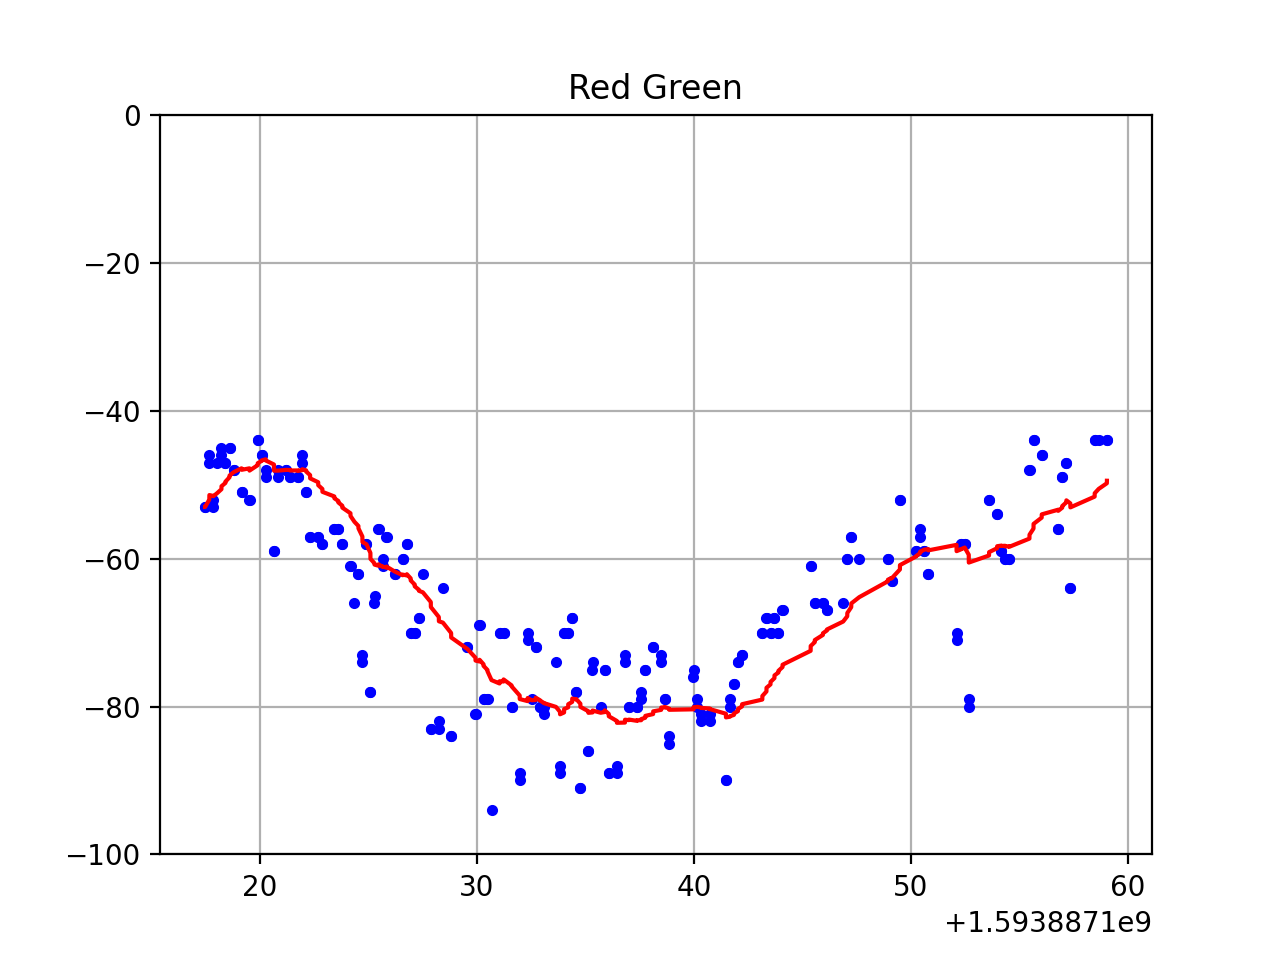
\includegraphics[width=1.0\textwidth]{Experiment-1-MBP-IGM.png}
    \caption{Experiment \#1 - MacBook Pro, Integrated Gauss-Markov}
    \label{fig:experiment-1-mbp-igm}
\end{figure}

Using the integrated Gauss-Markov model on the data of the second experiment for
the UUID of the stationary iPhone produces the results shown in Figure
\ref{fig:experiment-2-iphone-igm}.

\begin{figure}[ht]
    \centering
    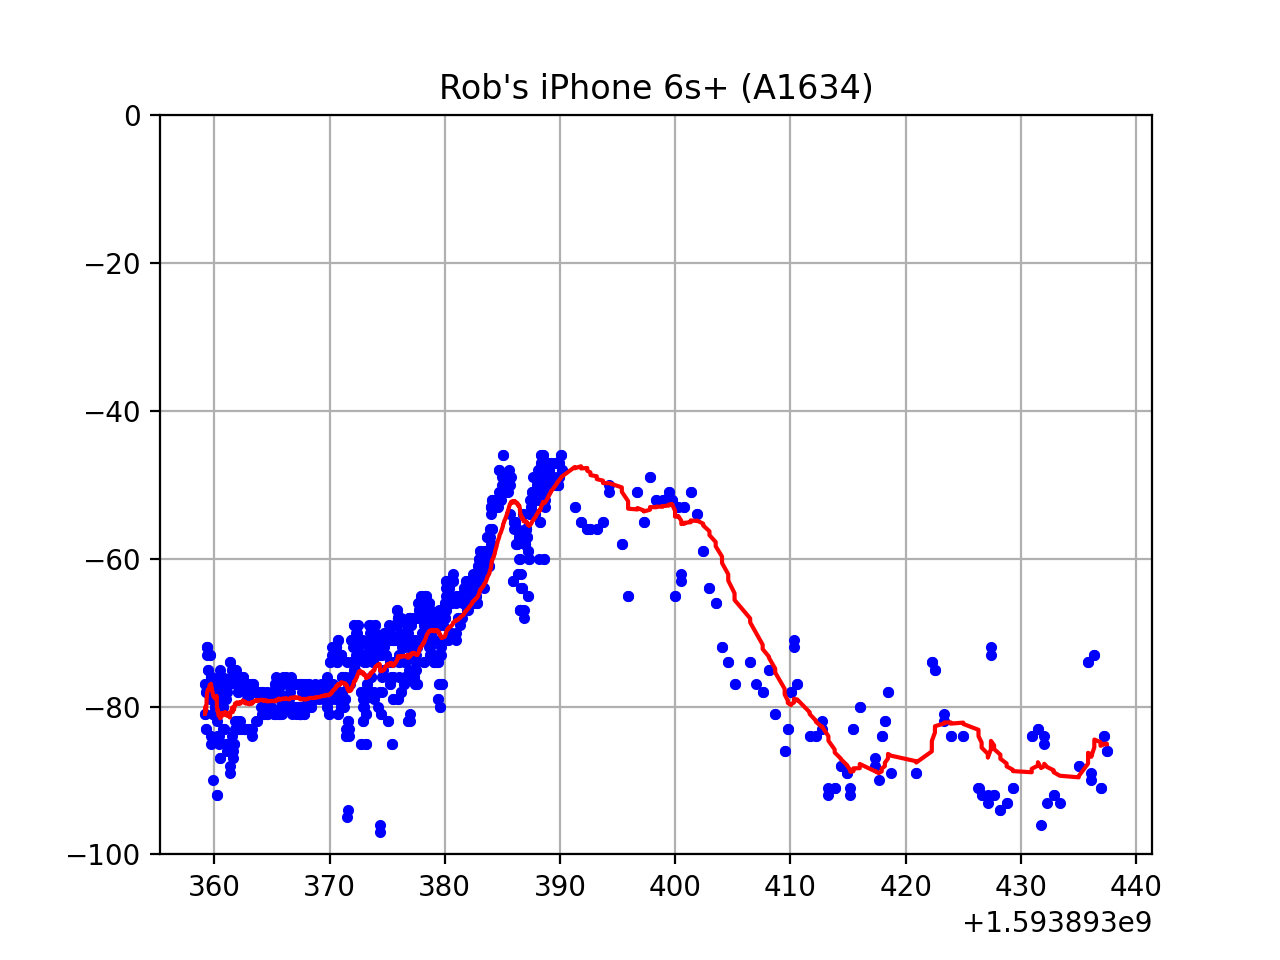
\includegraphics[width=1.0\textwidth]{Experiment-2-iPhone-IGM.png}
    \caption{Experiment \#2 - Stationary iPhone, Integrated Gauss-Markov}
    \label{fig:experiment-2-iphone-igm}
\end{figure}

Unlike the results of the Gauss-Markov with random bias model, it definitely appears that
the integrated Gauss-Markov model offers a substantial improvement over the Gauss-Markov
model. The filtered estimate is much more centered within the RSSI measurement data than
that of the Gauss-Markov model, and the filtered estimate is smoother yet still responsive.
The added processing complexity in going from a scalar filer to a $2 \times 2$ matrix
filter is worth the the effort for the use of this filter model for this particular
application. In fact, because it is a two-state filter, the matrix operations can be
explicitly coded for each element, thereby improving efficiency.

For completeness, the back yard results for the MacBook Pro can be seen in Figure
\ref{fig:experiment-2-mbp-igm}, and the results for the Apple TV can be seen in Figure
\ref{fig:experiment-2-atv-igm}.

\begin{figure}[ht]
    \centering
    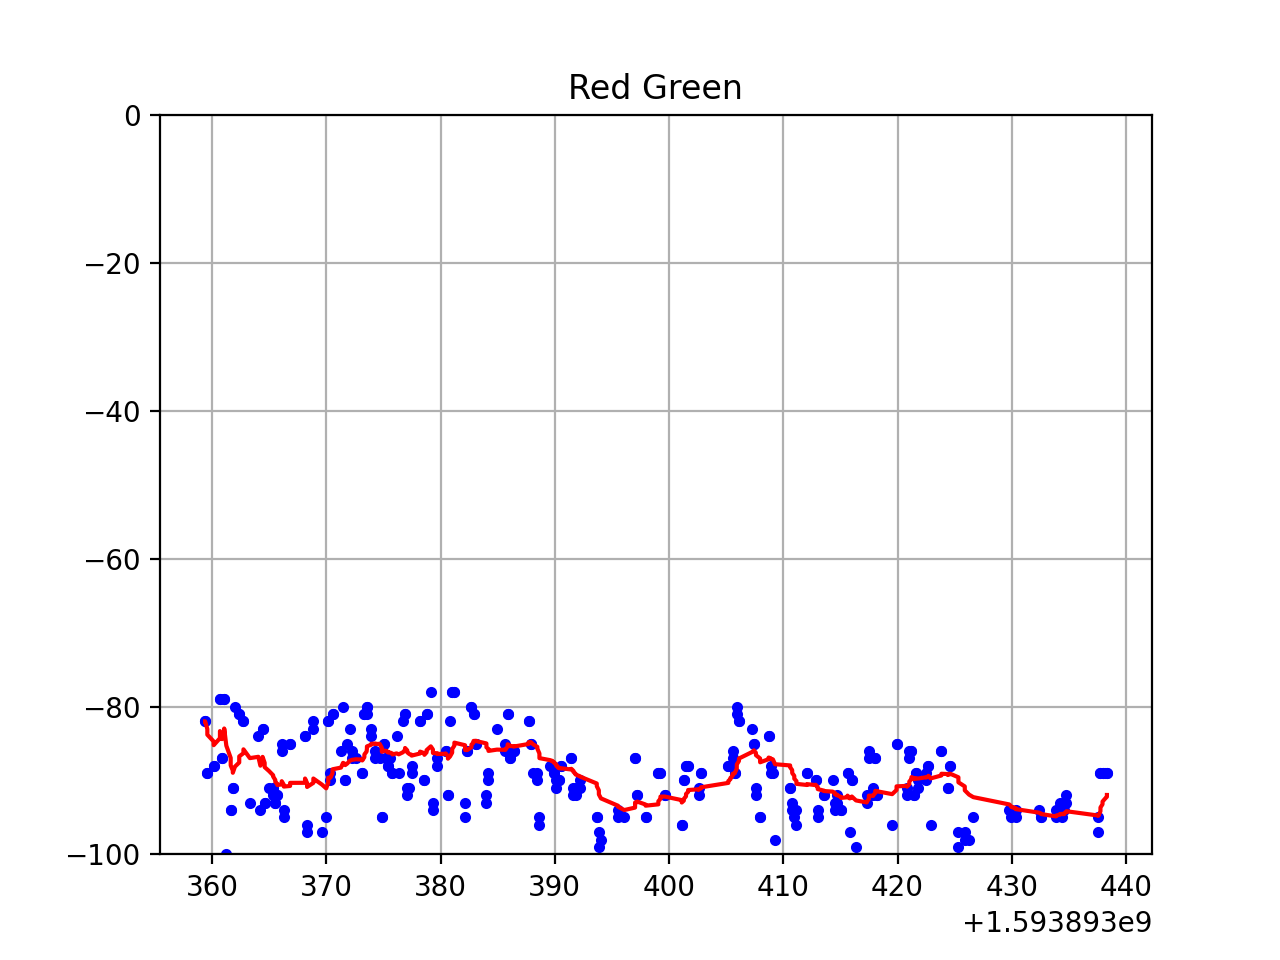
\includegraphics[width=1.0\textwidth]{Experiment-2-MBP-IGM.png}
    \caption{Experiment \#2 - MacBook Pro, Integrated Gauss-Markov}
    \label{fig:experiment-2-mbp-igm}
\end{figure}

\begin{figure}[ht]
    \centering
    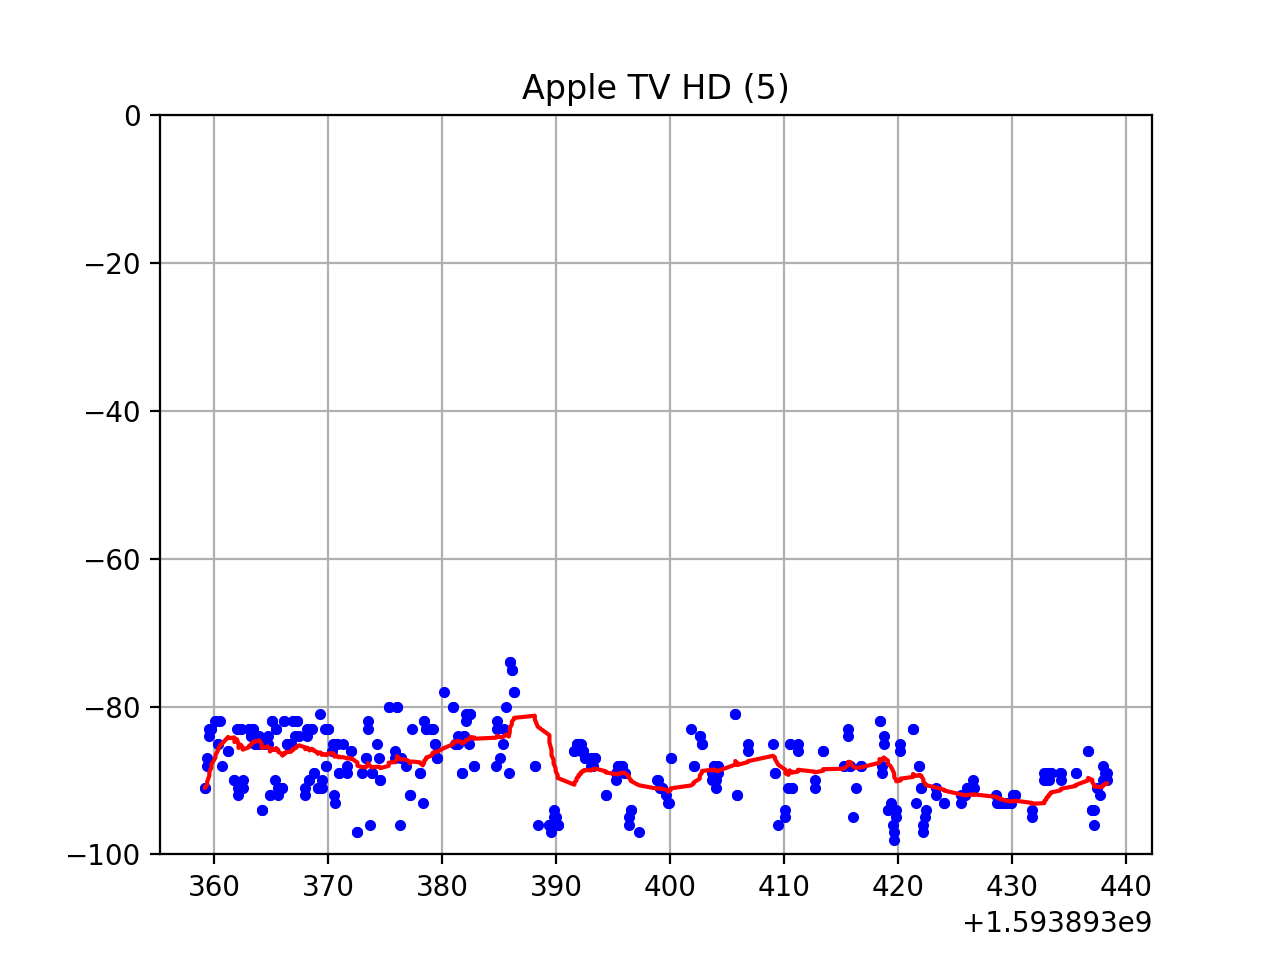
\includegraphics[width=1.0\textwidth]{Experiment-2-ATV-IGM.png}
    \caption{Experiment \#2 - Apple TV, Integrated Gauss-Markov}
    \label{fig:experiment-2-atv-igm}
\end{figure}



%-------------------------------------------------------------------------------
%
% Summary
%
%-------------------------------------------------------------------------------

\clearpage
\section{Summary}

It is evident that, for estimating RSSI signal levels acquired via a mobile device, the
integrated Gauss-Markov Kalman filter produces superior results over the Gauss-Markov
Kalman filter.
Figures \ref{fig:experiment-1-mbp-compare} and \ref{fig:experiment-2-iphone-compare}
illustrate this comparison.

\begin{figure}[!h]
    \begin{adjustbox}{max width=1.2\linewidth,center}
    \centering
    \begin{subfigure}{0.6\textwidth}
        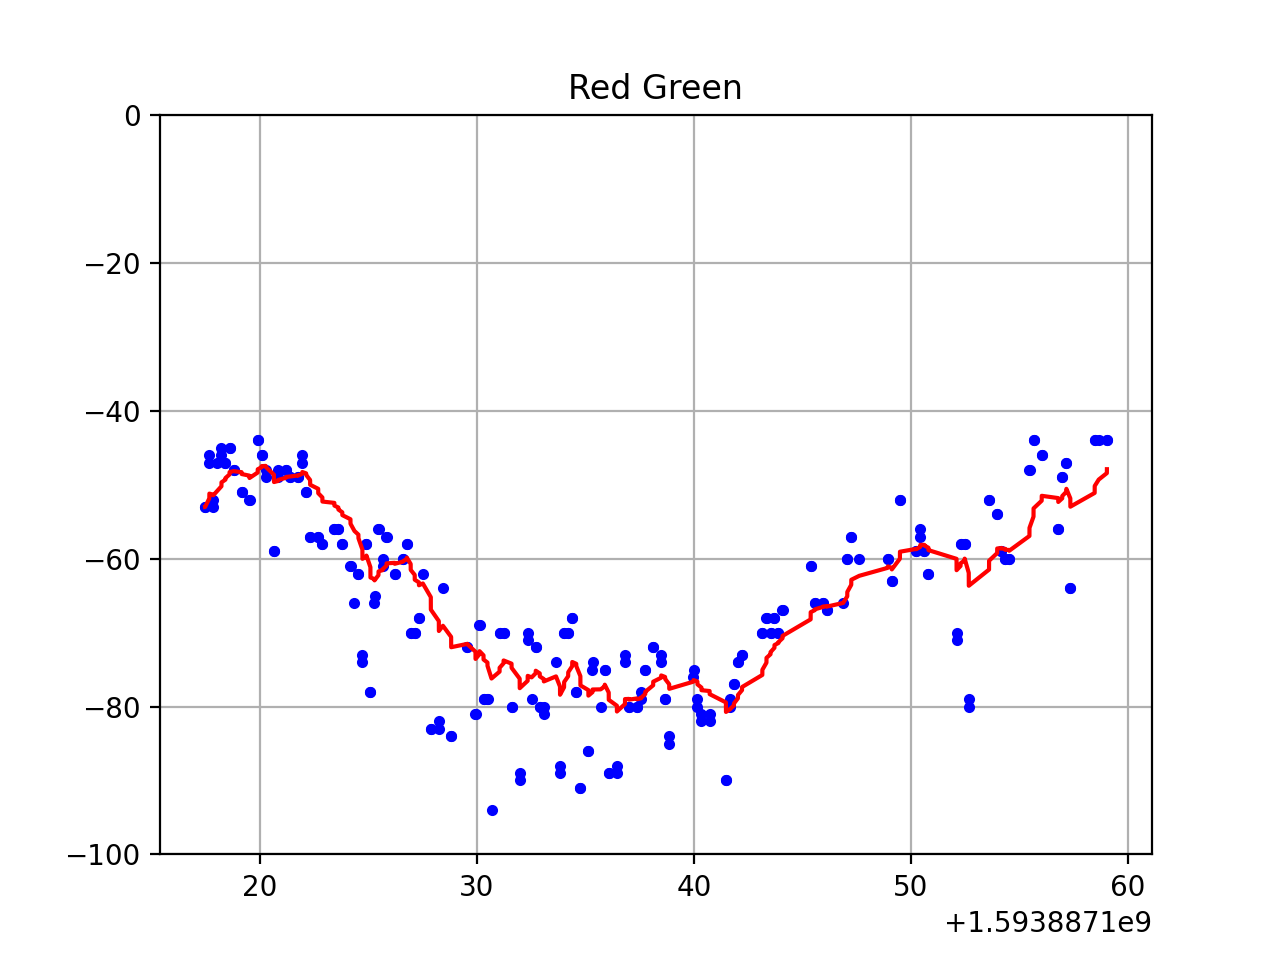
\includegraphics[width=\textwidth]{Experiment-1-MBP-GM.png}
        \caption{Gauss-Markov}
    \end{subfigure}
    \hskip -5ex
    \begin{subfigure}{0.6\textwidth}
        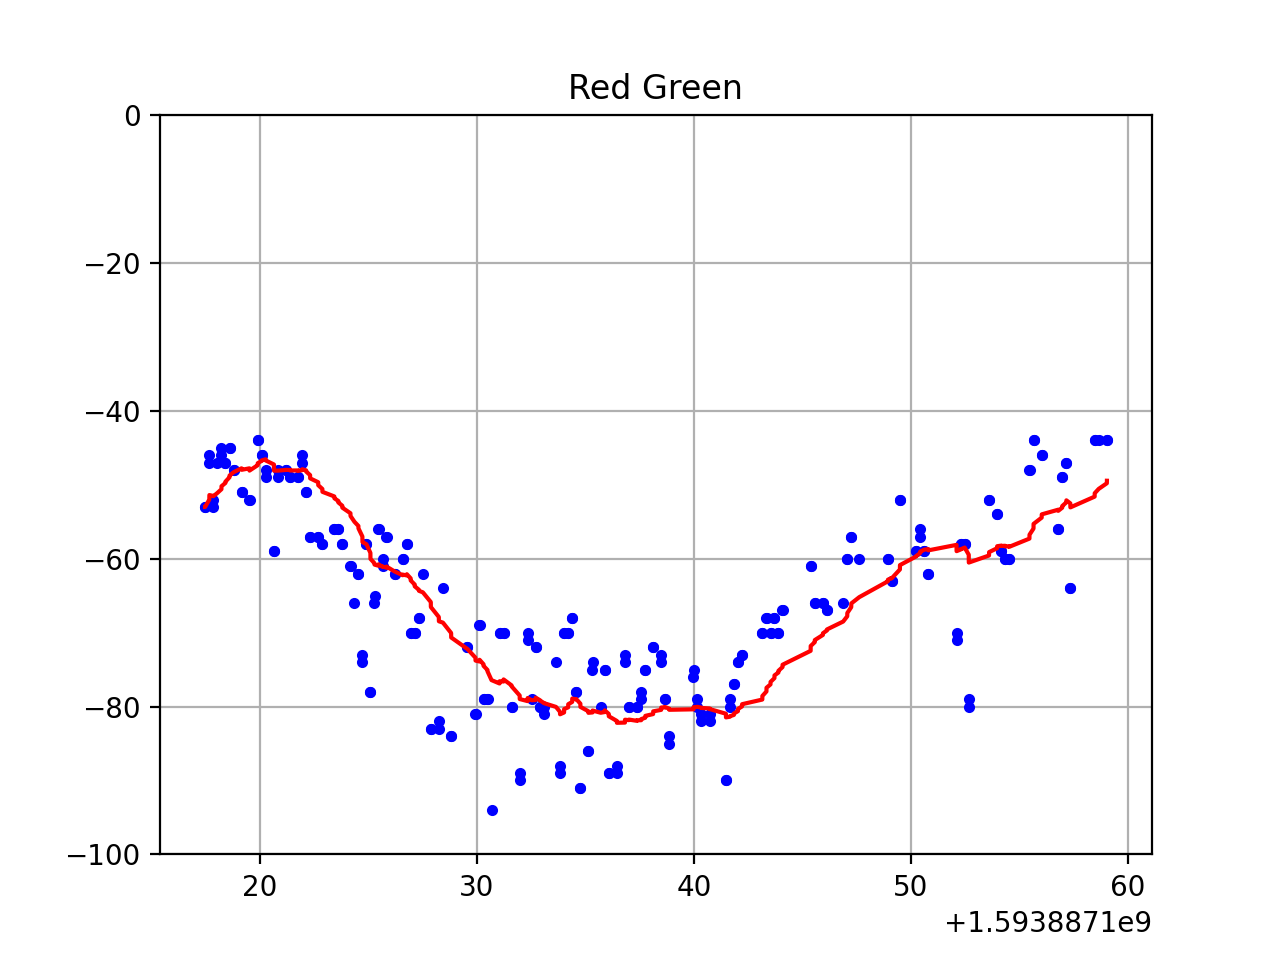
\includegraphics[width=\textwidth]{Experiment-1-MBP-IGM.png}
        \caption{Integrated Gauss-Markov}
    \end{subfigure}
    \end{adjustbox}
    \caption{Experiment \#1 Model Comparisons}
    \label{fig:experiment-1-mbp-compare}
\end{figure}

\begin{figure}[!h]
    \begin{adjustbox}{max width=1.2\linewidth,center}
    \centering
    \begin{subfigure}{0.6\textwidth}
        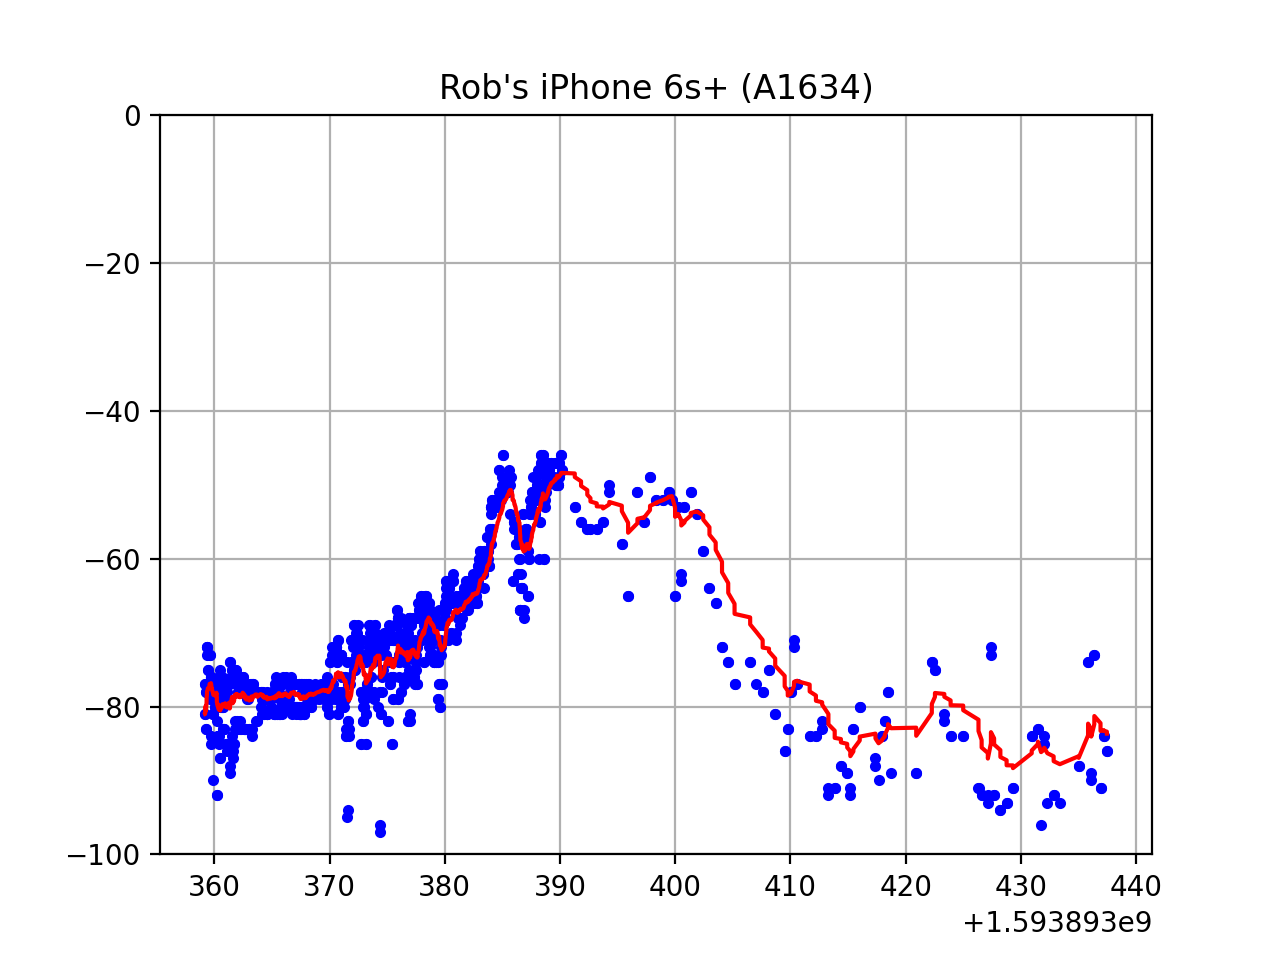
\includegraphics[width=\textwidth]{Experiment-2-iPhone-GM.png}
        \caption{Gauss-Markov}
    \end{subfigure}
    \hskip -5ex
    \begin{subfigure}{0.6\textwidth}
        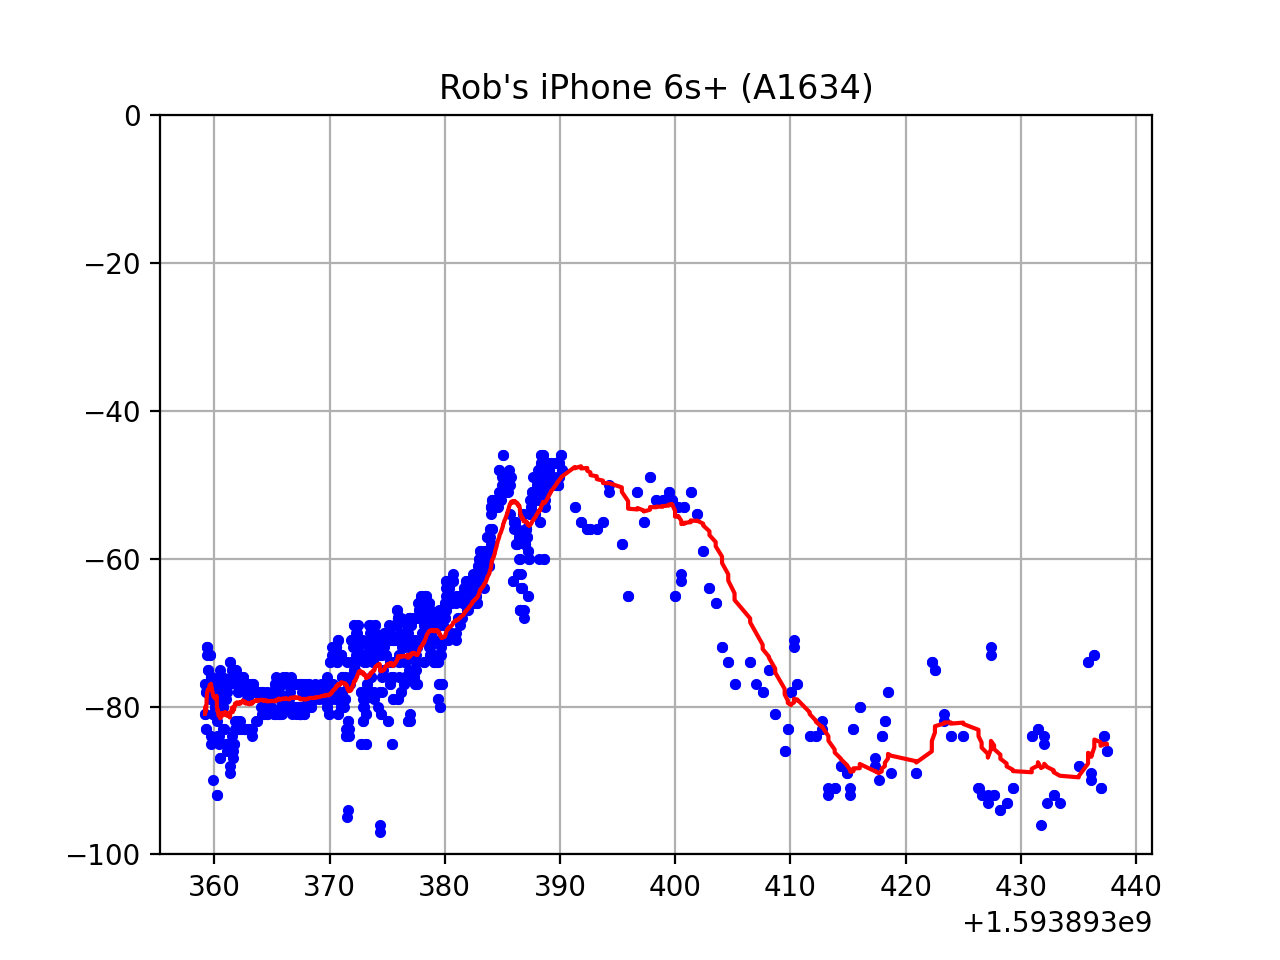
\includegraphics[width=\textwidth]{Experiment-2-iPhone-IGM.png}
        \caption{Integrated Gauss-Markov}
    \end{subfigure}
    \end{adjustbox}
    \caption{Experiment \#2 Model Comparisons}
    \label{fig:experiment-2-iphone-compare}
\end{figure}

\clearpage

While additional refining of tuning the filter parameters is needed before producing a
production-worthy filter, it can be concluded that the feasibility of using a Kalman
filter for estimating RSSI signal level is justified, and it is recommended that the
integrated Gauss-Markov process model be the preferred choice for implementation.

You can access the source for this project from my GitHub repo: \\
%\textcolor{blue}{https://github.com/rshuston/RSSISniffer}
\textcolor{blue}{\url{https://github.com/rshuston/RSSISniffer}}



%-------------------------------------------------------------------------------
%
% References
%
%-------------------------------------------------------------------------------

\clearpage

\begin{thebibliography}{9}

\bibitem{rgbrown1983}
Brown, R. G., 1983, \\
\emph{Introduction to Random Signal Analysis and Kalman Filtering},
John Wiley \& Sons, Inc., New York, NY.

\bibitem{sorenson1985}
Sorenson, H. W. (Ed.), 1985, \\
\emph{Kalman Filtering: Theory and Application},
IEEE Press, New York, NY.

\bibitem{chuichen1987}
Chui, C. K. and Chen, G., 1987, \\
\emph{Kalman Filtering with Real-Time Applications},
Springer-Verlag, New York, NY.

\bibitem{grewalandrews1993}
Grewal, M. S., and Andrews, A. P., 1993, \\
\emph{Kalman Filtering: Theory and Practice},
Prentice-Hall, Englewood Cliffs, NJ.

\end{thebibliography}

\end{document}
